\documentclass[12pt,a4paper]{article}
\usepackage[utf8]{inputenc}
\usepackage{url}
\usepackage{hyperref}
\usepackage{float}
\usepackage[utf8]{inputenc}
\usepackage[english]{babel}
\usepackage{url}
\usepackage{graphicx, capt-of}
\usepackage{titletoc}
\usepackage{setspace}   %Allows double spacing with the \doublespacing command
\usepackage{authblk}
\usepackage{float}
\usepackage{geometry}
\usepackage{textcomp}

\usepackage{caption}
%\geometry{legalpaper, margin=1.2in}
\usepackage[usenames, dvipsnames]{color}
 
%Import the natbib package and sets a bibliography  and citation styles
\usepackage{natbib}
%Import siunitx packages so that tables can be centered
\usepackage{siunitx} 
\usepackage{multirow}
\sisetup{
  round-mode          = places, % Rounds numbers
  round-precision     = 2, % to 2 places
}
\usepackage{rotating}
\usepackage{subcaption}
\usepackage[table]{xcolor}

\newcounter{subfloat}
\renewcommand{\thesubfloat}{\alph{subfloat}}
\newcommand{\image}[2]{%
  \stepcounter{subfloat}%
  \begin{tabular}[t]{@{}c@{}}
  #2 \\
  \end{tabular}%
}

\definecolor{lightgray}{gray}{0.9}
\definecolor{lightblue}{rgb}{0.93,0.95,1.0}

\begin{document}
\pagenumbering{gobble}
{\fontfamily{phv}\selectfont}
\title{\Huge Exploring the Landscape of Glycan Structure\vspace{1cm}\\ \large  MSc Bioinformatics and Theoretical Systems Biology Project\vspace{11cm}}
% * <steven.hargreaves17@ic.ac.uk> 2018-03-20T16:27:53.008Z:
% oh come on now...!
% ^.
\date{}
%\begin{figure}[!b]
%\centering 
%\includegraphics[width=0.5\textwidth]{images/2000px-Imperial_College_London_crest_svg.png}
%\end{figure}
%\begin{figure}[H]
%\centering
%\includegraphics[width=0.5\textwidth]{images/2000px-Imperial_College_London_crest_svg.png}
%\end{figure}
%\vspace{1cm}

\author{\Large Steven Hargreaves\\
\normalsize CID 01453122 \\\vspace{0.5cm}
\normalsize Imperial College London \\
\normalsize Department of Life Sciences}


\maketitle
%\setcitestyle{numbers}
\newpage
\begin{abstract}
\pagenumbering{arabic}
\doublespacing
contributions\\

- identify mis-laballed motifs\\

- we can determine glycan structure similarity\\
-- without needing to model the precise tree structure\\
-- so could also predict structure of unknown glycans from GE data or enzyme abundance\\

remove URLs from refs\\

use spell-checker\\

% \noindent RE-WRITE\\
% IMPOTANT - BEAR IN MIND THE EXAMINER WILL PROB ONLY SPEND ABOUT 20 MINS READING THIS, SO NEED TO GRAN THEIR ATTENTION AND CONVINCE THEM QUICKLY IN ABSTRACT AND INTRO. USE GOOD SUMMARY DIAGRAMS AND TEXT.\\
% Include some numbers for Sternberg\\
% e.g. no. glycans (pre/post filtering steps), no. motifs, assortativity coeffs?\\
% IMPORTANT - what's my contribution?\\
% Each major new section (e.g. Methods) should start on a new page\\
% The project report must include the word count on the title page (the number of words will be checked and failure to comply with the word limit will incur penalties)\\
% critically evaluated your results\\
% The Abstract
% should be structured (i.e. aims, methods, results, conclusion), be no more 
% than  one  side  of  paper  (in  written  reports).  Ideally  the  Abstract  should  cite  some  key numerical  results  rather  than  just  generalities.    Making  a  point  in  an  abstract  does  not remove  the  requirement  for  it  to  be  made  elsewhere  in  the  report.  The  report  must  be comprehensible even if the abstract is removed.  \\
% etc. etc. - see course handbook\\
% Glycans are tree-like polysaccharides that are frequently found attached to specific sites on eukaryotic cell surface and cellular matrix proteins, with diverse functions including protein folding, cell-cell signaling and immune response. Large databases describing observed glycan structures are now available, which provide an excellent resource for describing and exploring the space of naturally occurring glycans. In this project you will apply tree kernel methods to calculate distances between these structures and thereby develop clustering and data reduction methods to capture the most important differences between subsets of glycans, such as those observed in cancerous vs non-cancerous tissue.
\end{abstract}

\newpage
\begin{center}
\section*{Acknowledgements}
\doublespacing
Many thanks to John Pinney for his supervision and guidance during this project, and Suhail Islam for technical assistance. Database and JSON file icons used in Figure \ref{fig:flowchart} designed by Smashicons from Flaticon.
\end{center}
\newpage
\tableofcontents
\newpage
\section*{Abbreviations}
\doublespacing
\textit{RDF:} Resource Description Framework\\
\textit{SPARQL:} A recursive acronym for SPARQL Protocol and RDF Query Language\\
\addcontentsline{toc}{section}{Abbreviations} %adds it to the table of contents

\newpage
\section*{Glossary}
\addcontentsline{toc}{section}{Glossary}
\label{sec:glossary}
\doublespacing
% \noindent{\textit{Clade:} Blah.}\\\\
% \textit{Phylogenetic tree:} Blah blah.\\\\
% \textit{Archeopteryx.js:} ...phylogenetic trees .\\\\













\newpage
\section{Introduction}
\label{sec:intro}

% ** Max 12 figures and tables\\

% - Set in context of related research here. Don't mention \textit{Drosophila}



% - Describe glycans:\\

% As a minimum, say -- Glycans are chains of sugars, forming tree structures, with links like (blah), which can be alpha/beta etc. They're found (blah), and are used in cell signalling (and blah).\\

\subsection{Glycans}
\label{sec:glycans_description}
Monosaccharides are carbohydrates which cannot be further hydrolyzed to simpler compounds, such as glucose, fructose, and galactose. Glycans, synonymous with polysaccharides, are compounds of monosaccharides (usually more than ten) linked glycosidically \citep{mcnaught1997compendium}, which exist in free form or in covalent complexes with proteins or lipids \citep{doi:10.1093/bioinformatics/btm090}. In both cases, glycans exhibit a tree-like structure, which can be described in terms of its component monosaccharides and the glycosidic links between them. Figure \ref{fig:example_glycan} shows an example glycan, in which the differently coloured and shaped nodes represent different monosaccharides, and the labelled edges represent the glycosidic links (see \path{https://www.ncbi.nlm.nih.gov/glycans/snfg.html} for a list of monosaccharide symbols).

\begin{figure}[H]
\centering 
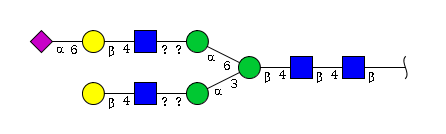
\includegraphics[scale=0.8]{images/glycan_G31576LD.png} 
\caption{An example glycan diagram. The differently coloured and shaped nodes represent different monosaccharides, and the labelled edges represent the glycosidic links between them (image taken from the GlyTouCan repository\protect\footnotemark). Glycosidic links are characterised by the anomericity ($\alpha$ or $\beta$) of carbon 1 on the first monosaccharide, and the carbon number of the non-anomeric carbon on the second monosaccharide. In a number of published glycans, the nature of some glycosidic links has not been satisfactorily established, and is therefore denoted as ambiguous via the use of question mark characters.}
\label{fig:example_glycan}
\end{figure}

\footnotetext{\url{https://glytoucan.org/Structures/Glycans/G31576LD}}

When dissolved in an aqueous environment, the monosaccharides (or sugars) of which glycans are comprised, primarily exist in the cyclic (or hemiacetal) form. In this form, the sugars are further characterised by their anomeric \mbox{configurations -- either} the $\alpha$-anomer, with an axial OH-group at carbon 1, or the $\beta$-anomer, with an equatorial OH-group at carbon 1 \citep{SONG2012137}. The glycosidic links between the sugars exist between carbon 1 (the anomeric carbon) of one sugar, and some other, non-anomeric carbon of another. Hence the links are defined by their anomericity ($\alpha$ or $\beta$), and the carbon number of the non-anomeric carbon on the second sugar. This can be seen more clearly in Figure \ref{fig:example_glycan}, where, for example, the N-Acetyl-Neuraminic Acid (purple diamond) is glycosidically linked via its $\alpha$-anomer carbon 1 to carbon 6 of the D-Galactose (yellow circle), and therefore labelled as `$\alpha$ 6'. This anomericity is significant -- two pairs of monosaccharides glycosidically linked via the same carbons but with different anomeric configurations result in two stereochemically distinct disaccharides, as illustrated in Figure \ref{fig:glycosidic_linkage}. Here, the polymeric form of the maltose disaccharide (starch) is digestible by humans, whereas cellulose, formed from basic repeats of cellobiose, is not \citep{SONG2012137}.\\

% \image{maltose}
% {%
%   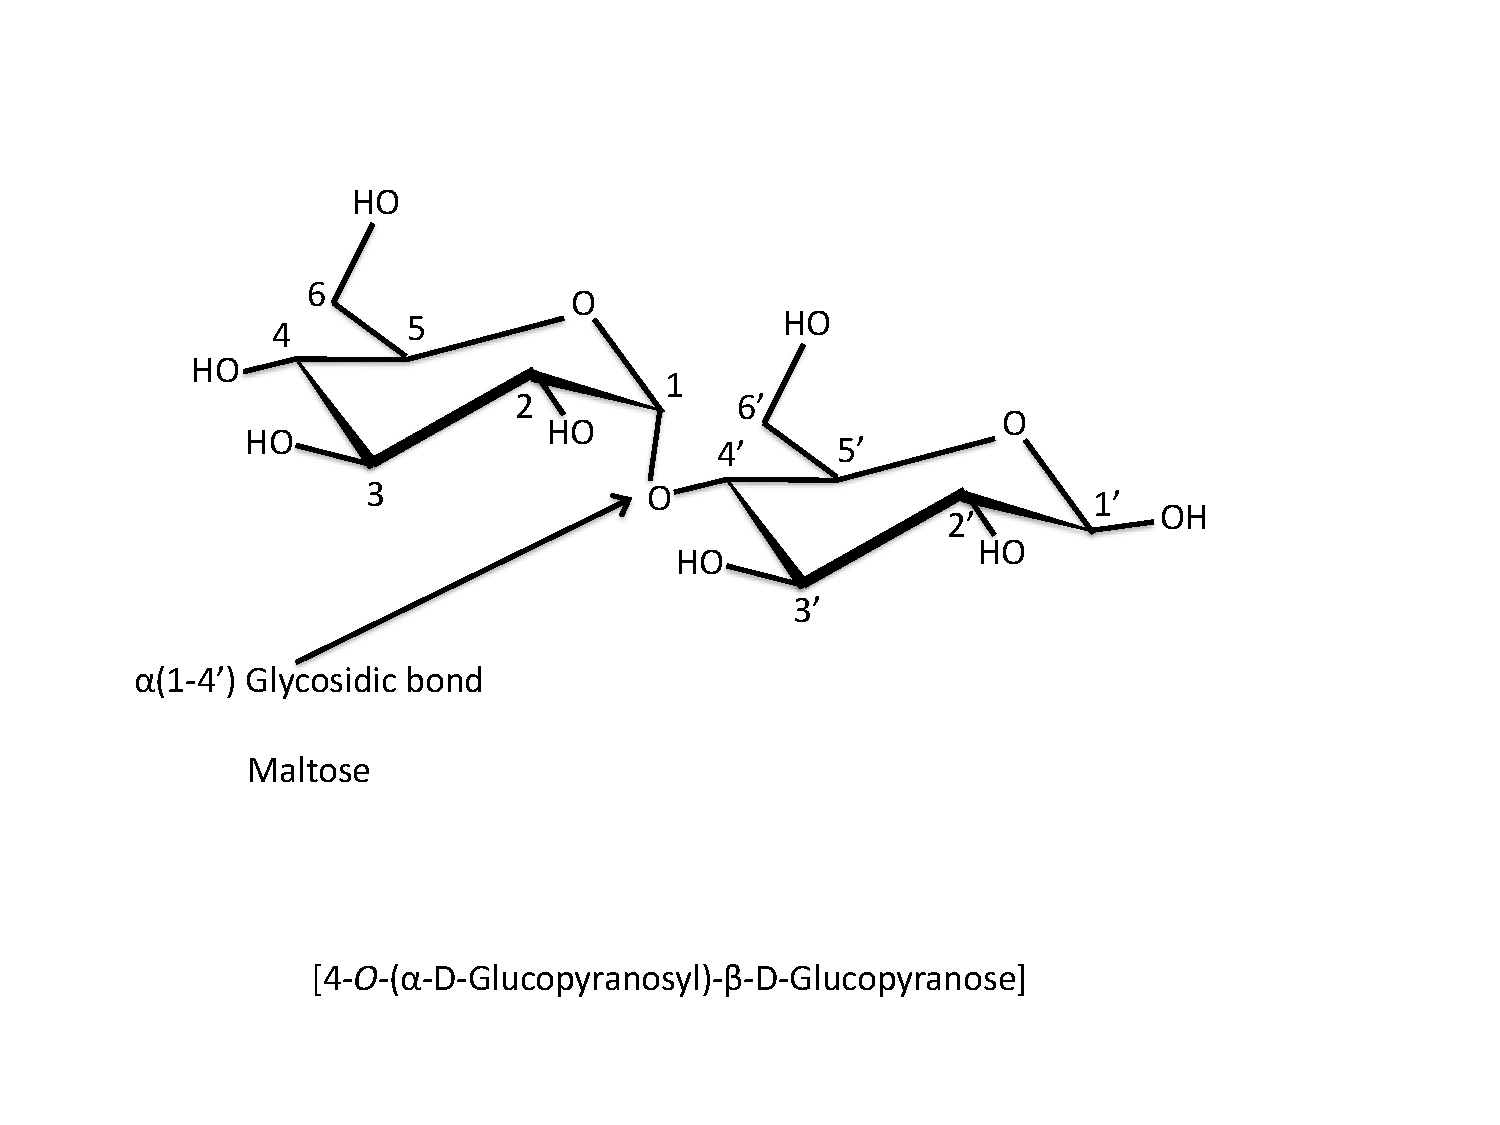
\includegraphics[scale=0.35]{images/glycosidic_linkage_maltose.pdf}%
% }\quad
% \image{cellobiose}{%
%   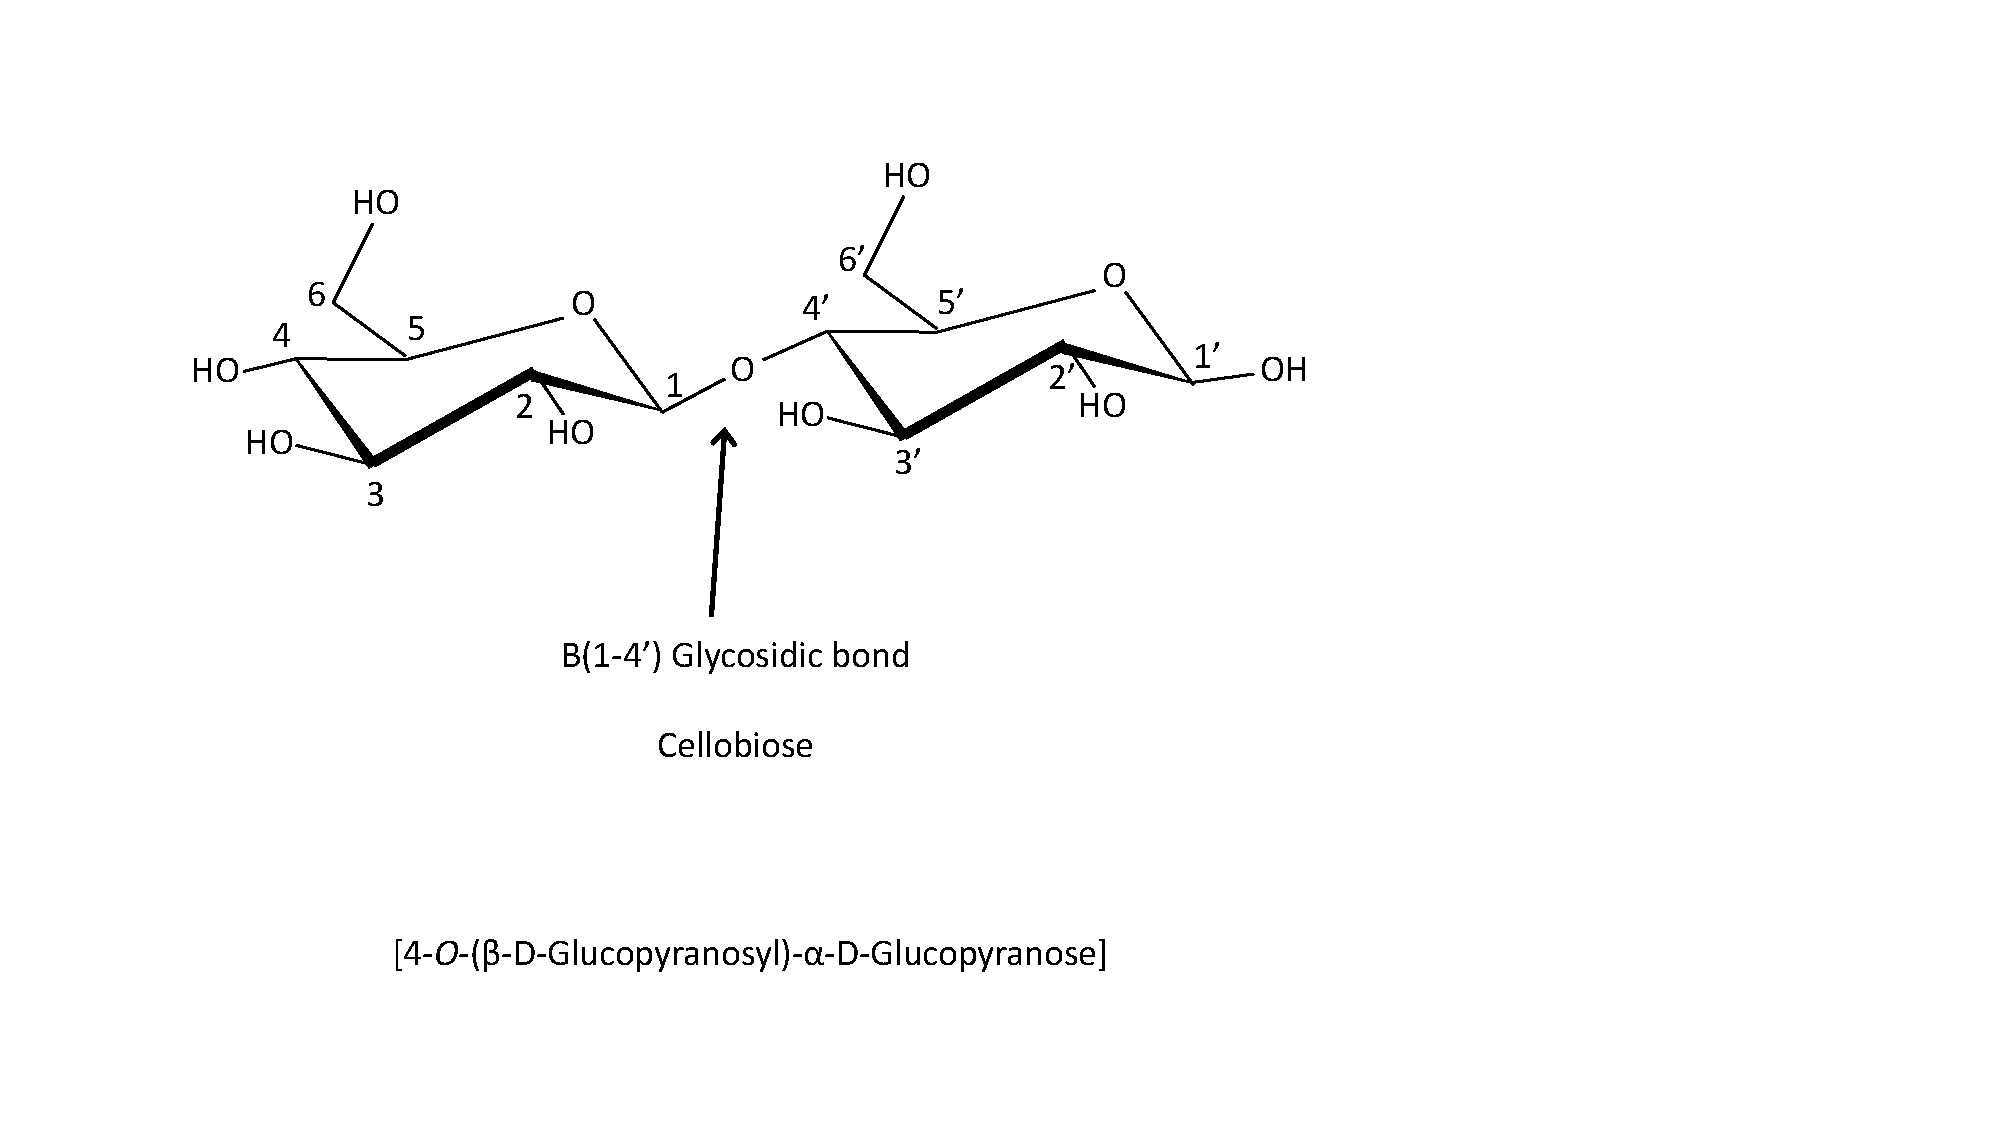
\includegraphics[scale=0.35]{images/glycosidic_linkage_cellobiose.pdf}%
% }\quad
% \captionof{figure}{CROP THESE PDFs, AND BRING THE O and HO closer together in the link.}
% \label{fig:glycosidic_linkage}

\begin{figure*}[ht!]
    \centering
    \begin{subfigure}[t]{1.0\textwidth}
        \centering
        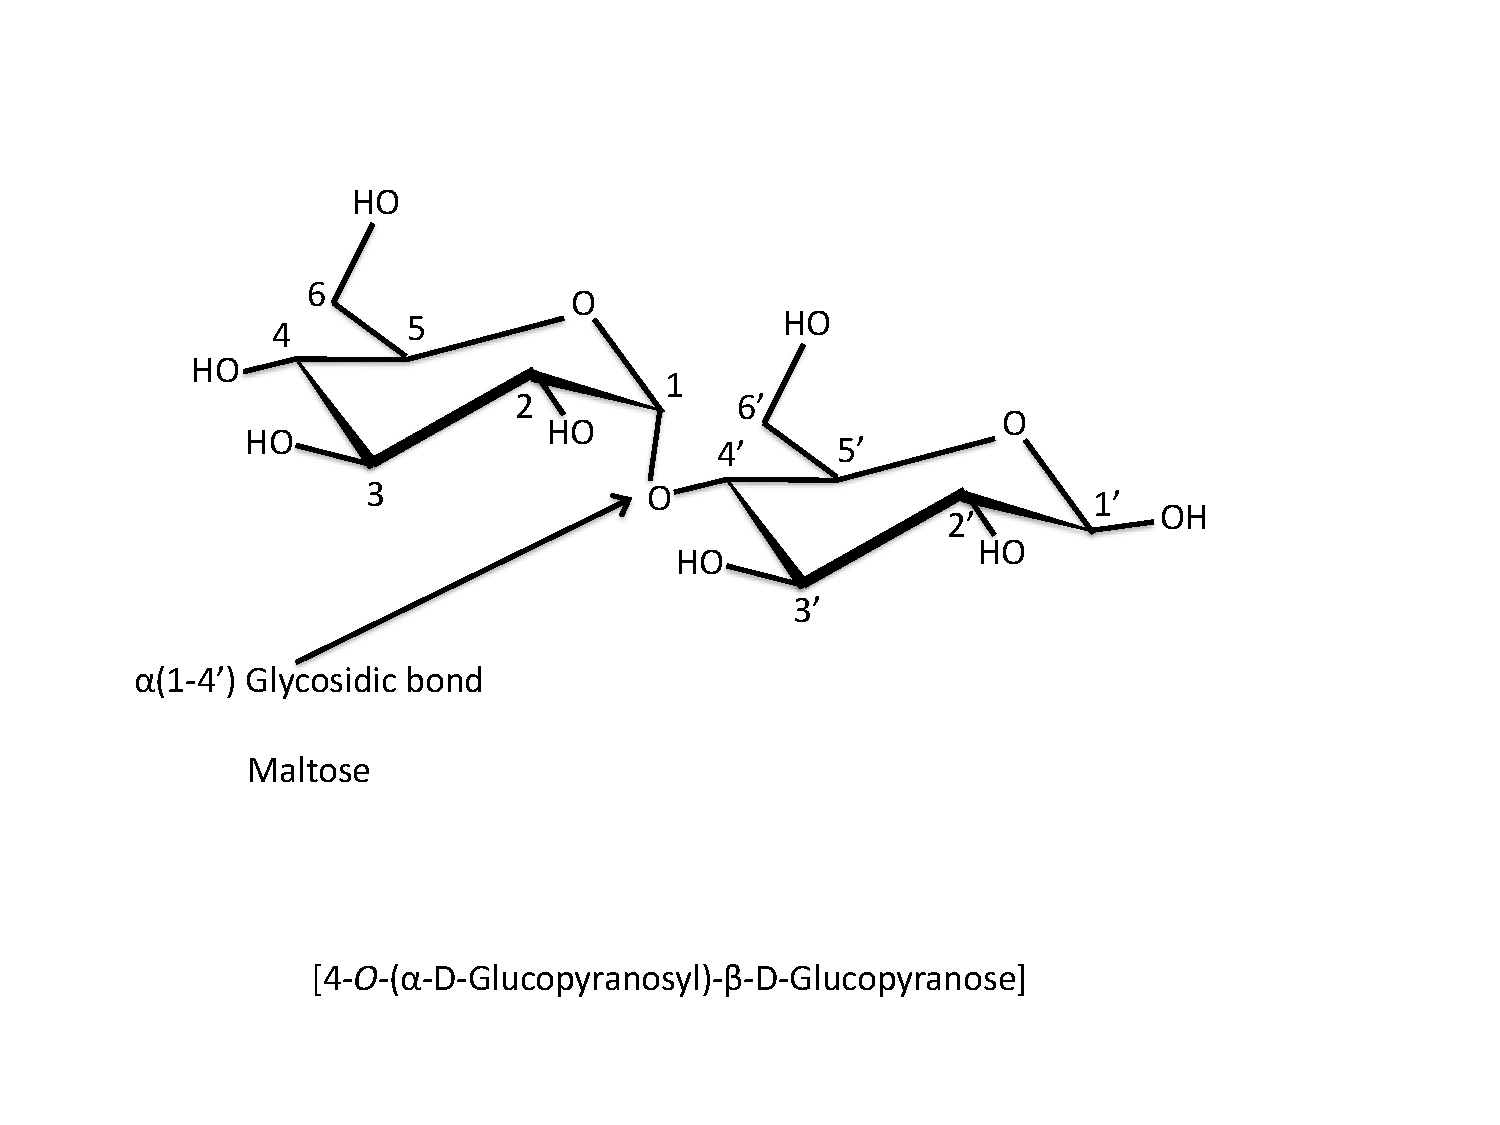
\includegraphics[scale=0.55]{images/glycosidic_linkage_maltose.pdf}
        \caption{Maltose}
    \end{subfigure}%
    \\
    \bigbreak
    ~ 
	\\
    \begin{subfigure}[t]{1.0\textwidth}
        \centering
        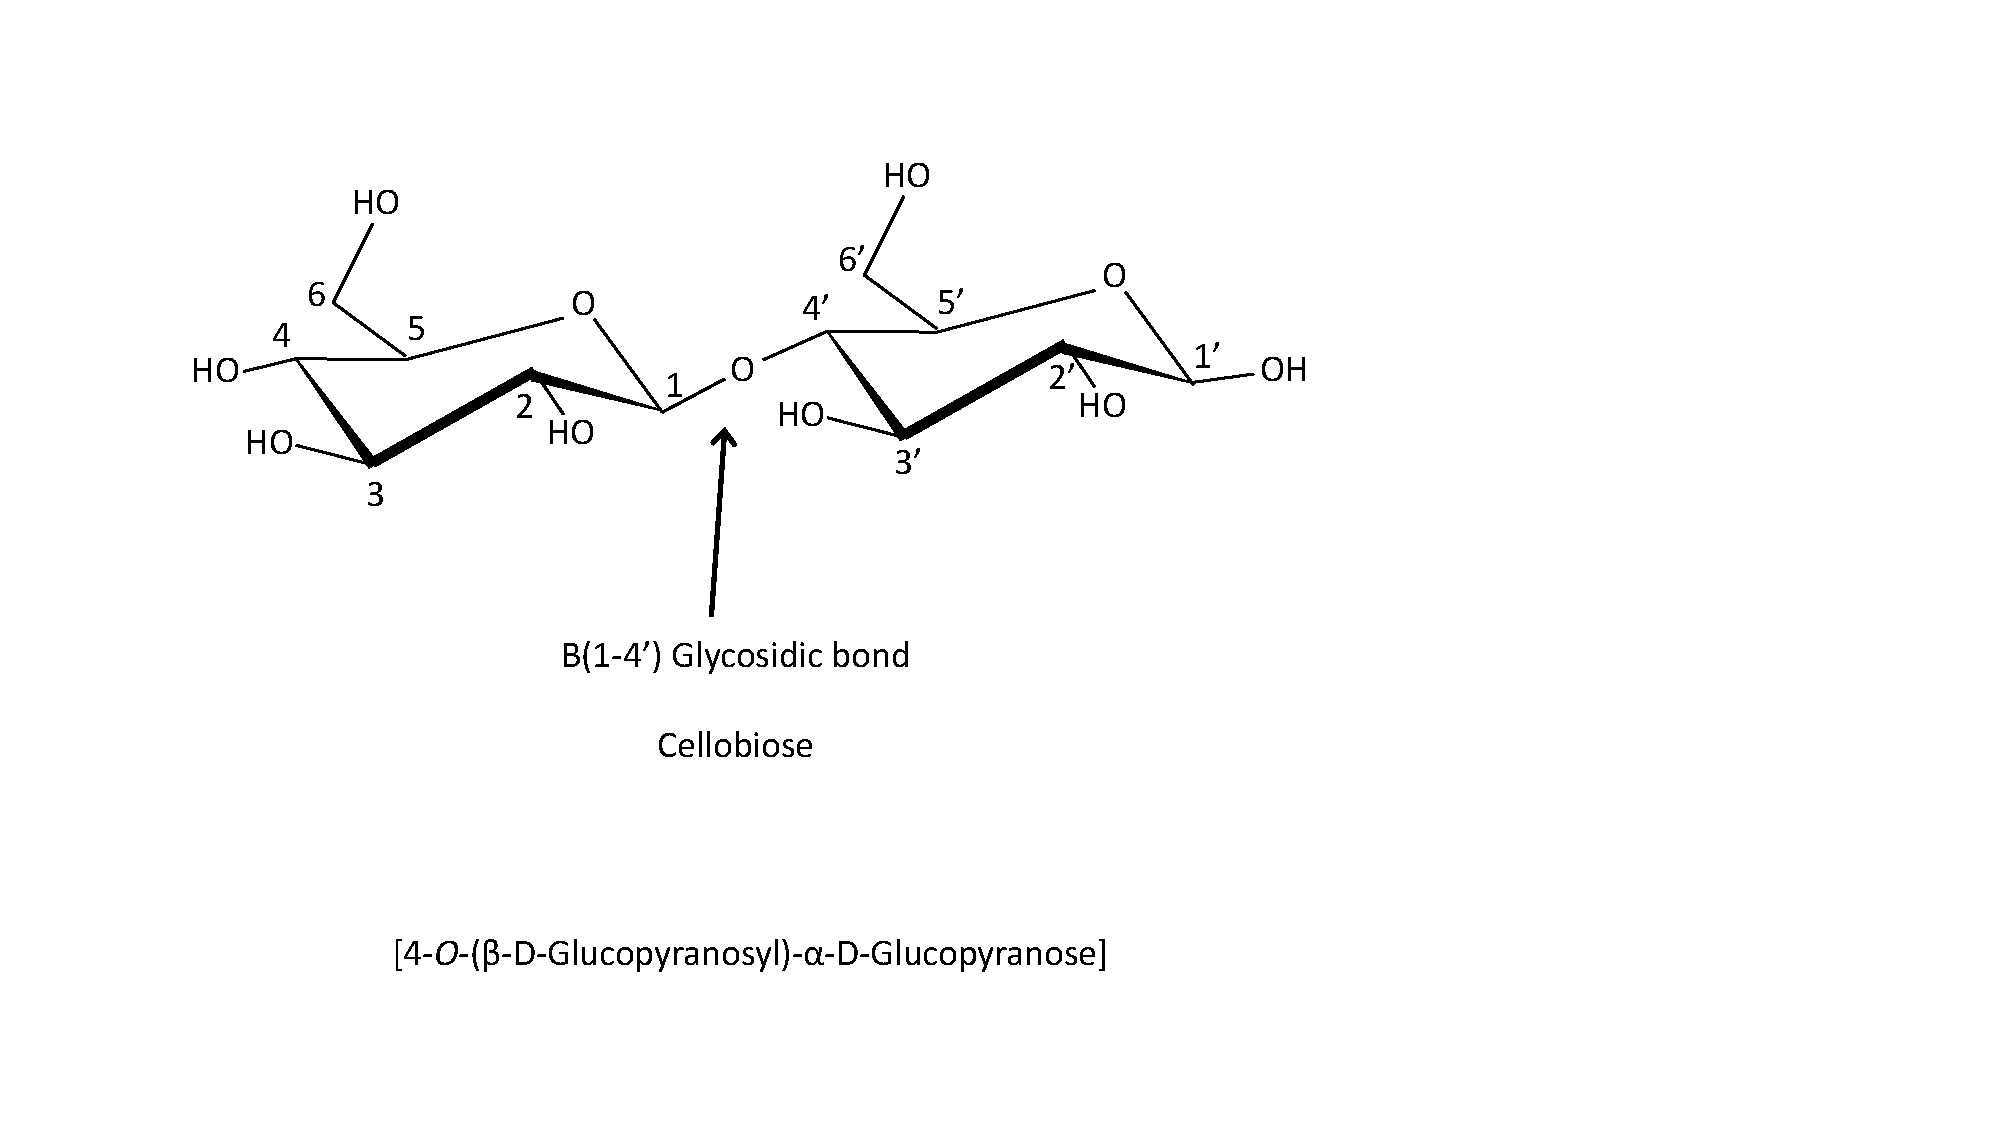
\includegraphics[scale=0.55]{images/glycosidic_linkage_cellobiose.pdf}
        \caption{Cellobiose}
    \end{subfigure}
    \caption{Pairs of the same monosaccharide (Glucose) glycosidically linked with different anomericity form different disaccharides (a) maltose and (b) cellobiose. Image based on Figure 4 from \citep{SONG2012137}.}
\label{fig:glycosidic_linkage}
\end{figure*}

When glycans are linked with proteins or lipids, they are characterised as being either N-linked, in which a monosaccharide is attached to a nitrogen atom of a protein \citep{taylor2011introduction}, or O-linked, in which a glycosidic oxygen links the glycoside to the aglycone or reducing end sugar (LOOK FOR AN ALTERNATIVE, CITABLE EXPLANATION OF THIS, E.G. IN ALBERTS OR THE BIG BIOCHEM BOOK).



% (from wikipedia, no citation - "Glycans can be found attached to proteins as in glycoproteins and proteoglycans. In general, they are found on the exterior surface of cells. O- and N-linked glycans are very common in eukaryotes but may also be found, although less commonly, in prokaryotes.")\\

% (more material on wikipedia if you need it)\\
% (lots of useful info here https://www.sciencedirect.com/science/article/pii/B9780444533494002466 including the chemistry of polysaccharides, which might be useful wrt using glycan reactions.)\\

% (Could also use "Sugars, Mono/poly-saccharide definitions in Alberts chapter 2, 'Biochemistry - The chemistry of Life' David Plummer chapter 3")\\














% -- Where do we find them\\
\subsection{Glycan Diversity, Locations and Motifs}
\label{sec:glycan_locations}
In contrast to the type of bonds found in proteins and nucleic acids, the high number of different glycosidic link configurations possible between monosaccharides leads to high variation and structural diversity between glycans, which confer distinctive characteristics to the cell surface where they are typically found \citep{10.1371/journal.pcbi.1002813}.
There are a total of 105050 distinct glycan structures present in the GlyTouCan\footnote{\url{https://glytoucan.org/}} database. Glycans do however share some common sub-structures, known as motifs. For example, the glycan structure represented in Figure \ref{fig:example_glycan} contains the `N-Glycan core basic' motif, which is displayed in Figure \ref{fig:N-Glycan core basic}. There are just 61 motifs presently listed in the GlyTouCan database - the full list (with diagrams) is available via the footnote link\footnote{\url{https://glytoucan.org/Motifs/listAll}}.

STATE / SHOW THE THREE MAJOR MOTIF TYPES (see wiki / glytoucan)

\begin{figure}[H]
\centering 
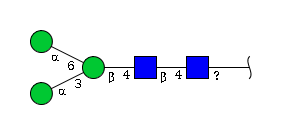
\includegraphics[scale=0.8]{images/n-glycan_core_basic.png} 
\caption{The `N-Glycan core basic' glycan motif, which can also be seen as part of the structure of the glycan shown in Figure \ref{fig:example_glycan}.}
\label{fig:N-Glycan core basic}
\end{figure}









% -- What do they do\\
\subsection{Glycan Function}
\label{sec:glycan_function}
Evidence has been found relating glycans to numerous important biological functions, including immune reaction, protein stabilization, and cell signalling \citep{bucior2004carbohydrate}, tumour progression \citep{fuster2005sweet}, and embryogenesis \citep{rosa2002functional}. Some pathogenic bacteria and viruses have been shown to infect their hosts via glycan-receptor interactions \citep{cossart2004bacterial, sacks2001molecular}, whilst other research has demonstrated that glycan profiles can represent important signatures of disease states \citep{tong2003glycosylation}.

% Recent research has revealed that these glycan profiles can represent important signatures of disease states and thus understanding glycan processing and structures in cells is an important systems biology goal \citep{10.1371/journal.pcbi.1002813}\\

% (glycans) draw attention as the third type of biological chain next to DNA and proteins, since they play key roles in many biological processes such as fertilization (Vo et al., 2003),  immunity (Rudd et al., 2001) and diseases (Birkle et al., 2003; Brockhausen et al., 1998; Hakomori, 2002). It is well known that some pathogenic bacteria and viruses infect their hosts via glycan-receptor interactions (Cossart and Sansonetti, 2004; Sacks and Kamhawi, 2001) \citep{doi:10.1093/bioinformatics/bti666}. \\

% Although a growing body of evidence supports crucial roles for glycans in many cellular processes, including cell-cell communication, immune system, protein interaction or tumor progression (Fuster and Esko, 2005; Varki et al., 1999), \citep{doi:10.1093/bioinformatics/btm090}

% (Glycans) are known to play numerous biological roles related to energy storage and metabolism, protein and lipid modification, cellular structure, signal transduction, as well as mediators of cell-cell interactions and host-pathogen interactions \citep{SONG2012137}




% -- Why are we interested\\

% -- How have they been analysed up until now, and what are the problems in analysing them\\
\subsection{Glycan Analysis}
\label{sec:glycan_analysis}

Given the important and diverse functions attributed to glycans, the ability not just to determine their individual structure, but also to accurately quantify their presence or absence within different cell and tissue types, is of great value. Methods of characterising glycan structures include mass spectral analysis \citep{10.1371/journal.pcbi.1002813}, high performance liquid chromatography, capillary electrophoresis, and nuclear magnetic resonance technology \citep{von2004bioinformatics}, whilst gene expression processing may be used to characterise glycosylation processing enzymes \citep{10.1371/journal.pcbi.1002813}.\\

Glycan analysis though remains highly problematic -- unlike the comparatively mature techniques regularly applied to DNA and RNA analysis, whose nucleotide chains are both linear and contain only 4 elementary components, and which are easy to amplify using (for example) polymerase chain reactions, glycans are tree-like in nature, and the large number of component monosaccharides involved together with the wide range of possible glycosidic links makes glycan structure determination challenging. Consequently only a small number of samples are available for analysis \citep{doi:10.1093/bioinformatics/bti666}.

To mitigate for these experimental shortcomings, in much the same way as sequence homology and multiple alignments may be exploited to construct complete genomes from DNA fragments (REF needed), there is a need for reliable computational techniques of glycan structure and prevalence prediction. Examples of research towards this end include probabilistic modelling of glycan families \citep{ueda2005probabilistic}, identification of glycan fingerprint differences between prostate cancer cell stages \citep{10.1371/journal.pcbi.1002813}, prediction of glycan structures from gene expression profiles \citep{doi:10.1093/bioinformatics/bti666}, and glycan comparison \citep{aoki2004score, aoki2004kcam} MAYBE A BIT MORE DETAIL ABOUT THESE TECHNIQUES AND RESULTS.




% To understand glycan functions, determination of their structures (sequences) like DNA and proteins is required. In spite of the improvements in purification and analytical methods for glycans such as high performance liquid chromatography, capillary electrophoresis, mass spectrometry and nuclear magnetic resonance technology (von der Lieth et al., 2004), the determination of the glycan structure is still difficult. Glycans have more complicated structures compared to nucleotide and amino acid sequences. While nucleotide and amino acid chains are linear and consist of 4 and 20 elementary components, respectively, glycan chains are branched structures and consist of various monosaccharides. In addition, they are multivalent, and linkages have anomeric configurations (alpha and beta). These complexities make it difficult to determine glycan structure. Furthermore, the amplification method of glycan is not yet fully established, while DNA and proteins are easy to amplify using polymerase chain reactions and cloning-expression systems, respectively. This means that only a few samples are available for glycan structure analysis. Therefore, a reasonable prediction method for glycan structures is useful for glycomics research. While the amino acid sequence of proteins is determined by the genetic code and the templates in the genome, the carbohydrate sequence of glycans is determined by the biosynthetic code, which is a specific set of biosynthetic reactions catalyzed by different types of glycosyltransferases (GTs). Each GT catalyzes formation of a glycosidic-bond between the glycan precursor as an accepter and the nucleotide-activated sugar as a donor (Varki et al., 1999). Thus, once we know the repertoire of GTs in the genome, in the transcriptome or in the proteome, it should, in principle, be possible to predict the repertoire of possible glycan structures in an organism or at a specific stage of the cell (von der Lieth et al., 2004). Here, we construct a reaction pattern library consisting of bond-formation patterns of GT reactions to link genome to glycome, and we predict glycan structures from gene expression profiles.

% However, gene set on DNA chips is incomplete, and gene expression data is noisy. To obtain appropriate prediction result, we extract knowledge of glycan structure from the glycan database and apply it to our prediction method. In particular, a co-occurrence frequency of reaction patterns is calculated from the KEGG GLYCAN database, which is a comprehensive resource encapsulating the latest knowledge of glycans and a part of the KEGG resource containing genomic information and pathways (Kanehisa et al., 2004; Hashimoto et al., 2005a), and we use it together with the reaction pattern library. First, we evaluate the prediction method using virtual expression data generated from the KEGG GLYCAN database. Then, we apply our method to publicly available DNA microarray expression data and find characteristic glycan structures in a particular cell. (Results) First, we constructed a reaction pattern library consisting of bond-formation patterns of GT reactions and investigated the co-occurrence frequencies of all reaction patterns in the glycan database. This was followed by the prediction of glycan structures using this library and a co-occurrence score. A penalty score was also implemented in the prediction method. Then we examined the performance of prediction by the leave-one-out cross validation method using individual reaction pattern profiles in the KEGG GLYCAN database as virtual expression profiles. The accuracy of prediction was 81\% \citep{doi:10.1093/bioinformatics/bti666}. \\

% Understanding the biological functions of glycans and relating them to their structure remains challenging experimentally. Unlike genes or protein sequences, for which a number of well-established algorithms are now available for various data-mining tasks such as similarity detection, clustering, supervised classification, structure prediction or functional motif extraction, glycans are generally not linear polymers. They have more complex structures, that can be represented by rooted ordered trees, with monosaccharides as labeled vertices and sugar bounds as labeled edges. As a result, specific approaches have recently been developed for comparison of glycans (Aoki et al., 2004, 2005), probabilistic modeling of glycan families (Ueda et al., 2005), and analysis of MS/MS spectra of oligosaccharides (Tang et al., 2005). There is still an incentive to develop efficient methods for the automatic classification of glycans, and the extraction of biologically relevant substructures. Glycans exhibit a large diversity of structures in different organisms, and in different tissues and organs of a given organism. Recently, a computational approach to the supervised classification of glycans into blood components and to the detection of leukemia-specific glycan substructures has been proposed (Hizukuri et al., 2005). The approach is based on the extraction of short linear substructures from the glycan structures, resulting in a quantitative measure of similarity between glycans based on the count of shared substructures. This measure of similarity is then used as an input to a support vector machine (SVM) classifier which is trained to discriminate between different blood components and blood types. The goal of this article is to extend this framework to a broader class of structure representations, with the motivation of both increasing the accuracy of glycan classification, and providing a framework for the extraction of biologically relevant glycan substructures.

% More precisely, we investigate different high-dimensional representations for glycan structures and use them for supervised classification with SVM. In SVM jargon, we define new kernels for trees, adapted to the classification of glycans. Our tree kernels are based on the indexation of a glycan tree structure by a set of subtrees it contains. We investigate different variants in the definition of subtrees, in the importance placed on the depth of a subtree in the glycan tree, and in the size of the subtrees. In spite of their large dimensions, these vector representations are adapted to the supervised classification of glycans by kernel methods and in particular the SVM, in the spirit of earlier work on convolution kernels for tree structures (Collins and Duffy, 2001; Haussler, 1999). We perform a thorough analysis of the classification performance obtained by different representations on the problem of predicting the blood origin of glycans among leukemia cell, erythrocyte, plasma and serum. We then apply feature selection methods to find discriminative subtree motifs in glycans, and relate the selected substructures to biologically known facts. Finally, in order to combine the information provided by different representations we apply recently developed methods for multiple kernel learning (Bach et al.,2005), resulting in an optimal weighting of each representation for each classification task. As shown in Section 4, the methods developed in this article not only lead to better classification performance than previously reported results, but also provide additional biological insights in the role and structure of glycans, through the substructures extracted by feature selection and the weights learned by multiple kernel learning. The proposed methods are tested on their ability to classify human glycans into four blood components: leukemia cells, erythrocytes, plasma and serum. They are shown to outperform a previously published method. We also applied a feature selection approach to extract glycan motifs which are characteristic of each blood component. We confirmed that some leukemia-specific glycan motifs detected by our method corresponded to several results in the literature \citep{doi:10.1093/bioinformatics/btm090}.\\

--- describe/list existing databases?\\


% -- What do we propose to do here, and why/how will it be helpful\\
\subsection{Proposed Method for Exploring the Landscape of Glycans}
\label{sec:proposed_method}
Intrinsic to the method of predicting of glycan structures from gene expression profiles cited above \citep{doi:10.1093/bioinformatics/bti666}, is a recognition of the fact that a specific set of glycosyltransferases (GTs) are required to catalyze the reactions necessary for synthesising specific glycans. By building a library of the bond formation patterns of GT reactions, and determining a co-occurence score of the reaction patterns in a glycan database, the authors predicted glycan structures with an accuracy of 81\%. Additionally, using gene expression data from the human carcinoma cell, the authors predicted the presence of sialic acid and the Sialyl Lewis X motif.

Expanding upon that approach, in this paper we describe a method of exploring glycan similarity from biochemical reaction similarity. More specifically, to compare any two glycans we calculate the Jaccard distance between the two sets of biochemical reactions necessary for the synthesis of each glycan in the pair. We visualise clusters of similar glycans via the use of networks, which allows us to explore whether or not glycans which we have judged to be similar in terms of their biochemical synthesis reactions are also similar in terms of their constituent motif sets. Furthermore, we perform hierarchical clustering using the Unweighted Pair Group Method with Arithmetic Mean (UPGMA), allowing us to form a dendogram / cladogram ???, from which we compare the groups of similar glycans found using the two alternative methods - THIS NEEDS RE-THINKING - SAY MORE ABOUT REACTIONS, INCLUDE A DIAGRAM LIKE Figure \ref{fig:gt_reaction_pattern}.

\begin{figure}[H]
\centering 
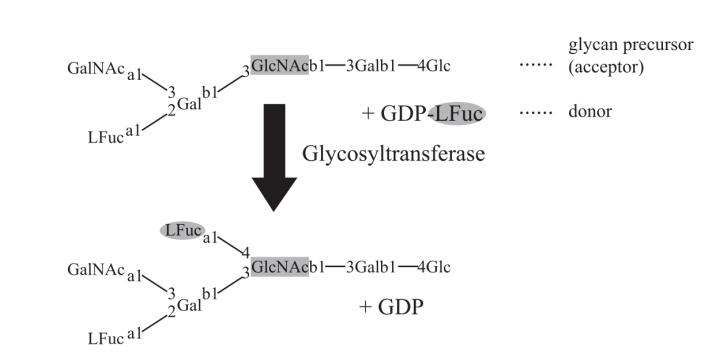
\includegraphics[scale=0.8]{images/gt_reaction_pattern.png} 
\caption{NEED TO RE-DRAW THIS}
\label{fig:gt_reaction_pattern}
\end{figure}

The rest of this paper is organised as follows -- in Section \ref{sec:method} we describe, in sufficient detail for a Bioinformatician or Computer Scientist to be able to reproduce our results, the databases and computational methods used, before presenting and discussing our results in Section \ref{sec:results}. In Section \ref{sec:discussion} we discuss our findings within the bigger picture of glycan analysis, before providing suggestions for further work and our conclusions in Sections \ref{sec:further_work} and \ref{sec:conclusions} respectively.


\subsection{MAKE SURE YOU'VE GOT ALL OF JOHN'S REFS IN. AND ALSO THE MOTIF PAPER cwp187.pdf}







% \subsection{Objectives}
% \label{sec:objectives}
% Do I want this bit?\\
% Formally, we state here the objectives of the project:
% \begin{enumerate}
% \item Objective 1.
% \item Objective 2.
% \end{enumerate}

% You can swap to singlespace for a list like this and back to doublespace afterwards:

% \singlespace
% \begin{enumerate}
% \item {\bf dndTree.js} \small \url{http://bl.ocks.org/robschmuecker/7880033} \normalsize
% \item {\bf phylotree.js} \small \url{http://phylotree.hyphy.org/#} \normalsize
% \item {\bf Phylogenetic Tree of Life} \small \url{https://www.jasondavies.com/tree-of-life/} \normalsize
% \item {\bf d3.phylogram.js} \small \url{http://bl.ocks.org/kueda/1036776} \normalsize
% \item {\bf PhyD3} \small \url{https://phyd3.bits.vib.be} \normalsize
% \item {\bf IcyTree} \small \url{https://icytree.org} \normalsize
% \item {\bf EvolView} \small \url{http://www.evolgenius.info/evolview/#mytrees/} \normalsize
% \item {\bf Archaeopteryx.js} \small \url{https://github.com/cmzmasek/archaeopteryx-js} \normalsize
% \end{enumerate}
% \doublespace

% And here's Table \ref{tab:tree_vis_eval}.\\

% \begin{table}[h]
% \centering
% %\resizebox{\columnwidth}{!}
% \begin{tabular}{|l|c|c|c|c|c|c|c|c|c|} \hline
% \multirow{2}{*} & \multicolumn{8}{c|}{\bf Candidate} \\  \cline{2-9}
% {\bf Functionality} & {\bf 1} & {\bf 2} & {\bf 3} & {\bf 4} & {\bf 5} & {\bf 6} & {\bf 7} & {\bf 8} 	\\ \hline
% Handles phyloXML & n & n & n & n & y & n & y & y \\ \hline
% Code clarity & n & n & n & n & n & y & n & y \\ \hline
% {\bf Score} & {\bf 3} & {\bf 8} & {\bf 3} & {\bf 8} & {\bf 13} & {\bf 12} & {\bf 13} & {\bf 14} \\ \hline
% \end{tabular}
% \caption{Phylogenetic tree visualisation software evaluation results.}
% \label{tab:tree_vis_eval}
% \end{table}

\newpage
\section{Method}
\label{sec:method}

Figure \ref{fig:flowchart} illustrates, at a high level, the methods used in this research. In brief, we:

\begin{enumerate}
\item Extract glycan structure and motif information from a public Glycan database (GlyTouCan)
\item Save the data locally
\item Parse the structure data, extracting the collection of reactions necessary to construct each glycan
\item Use the Jaccard distance measure to determine similarity between all pairs of glycans in terms of their reactions collections
\item Convert the similarity measurements to binary similar / dissimilar by application of a threshold
\item Create, visualise, and explore a network of similar glycans 
\item Construct, visualise and explore a cladogram via the use of hierarchical clustering
\end{enumerate}

In the following sub-sections we describe each of these steps in more detail.

\begin{figure}[H]
\centering 
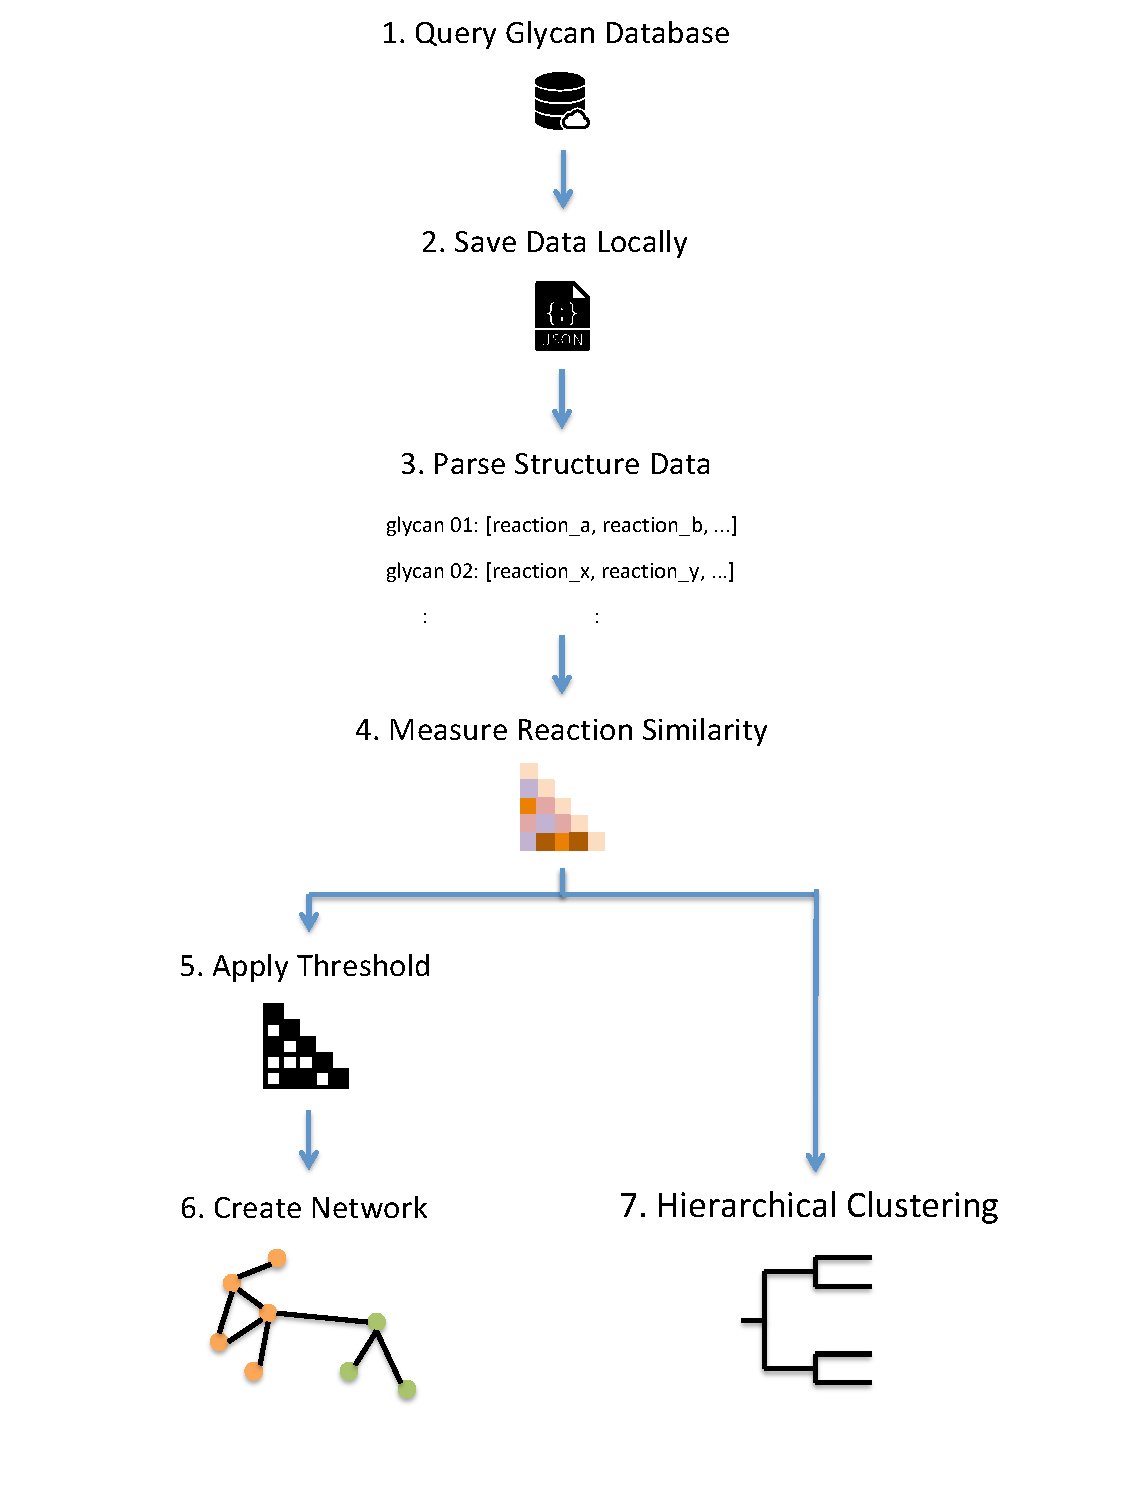
\includegraphics[scale=0.83]{images/flowchart.pdf} 
\caption{Method flowchart}
\label{fig:flowchart}
\end{figure}

\subsection{Reproducibility}
\label{sec:reproducibility}
The computer program code referenced throughout this report, and which was used to produce the results described, is available from a GitHub software repository. Details of how to obtain the code, as well as the Python package dependencies, can be found in Appendix \ref{sec:software_dependencies}. 

\subsection{Glycan Databases}
\label{sec:glycan_databases}

A number of different publicly accessible glycan databases exist, as well as multiple different formats for expressing glycan structure. The details of these databases and formats are listed in Tables \ref{tab:glycan_databases} and \ref{tab:glycan_format_counts} in Appendix \ref{sec:glycan_dbs_and_formats}. We use the GlyTouCan database, given its larger number of glycans and supported formats compared to the other databases, as well as the fact that it also contains motif information. In our trials it was also found to have the most suitable query method. We also chose to work with the Web3 Unique Representation of Carbohydrate Structures (WURCS) glycan structure format, which is the most recently devised format and which has been designed to address various shortcomings of the other existing formats \citep{matsubara2017wurcs}.

GlyTouCan is a semantic web graph database, rather than a relational database. Such databases contain Resource Description Framework (RDF) data, in which all data items take the form of \emph{triples}, and the database is queried using the query language SPARQL (a recursive acronym for SPARQL Protocol and RDF Query Language). A full description of this type of data is beyond the scope of this report, however some useful primers are available at the following URLs:

\singlespace
\begin{itemize}
\item RDF Primer \path{https://www.w3.org/TR/rdf11-primer/}
\item SPARQL 1.1 overview \path{https://www.w3.org/TR/sparql11-overview/}
\end{itemize}
\doublespace

The data we wish to extract from GlyTouCan is a list of glycan IDs, the text string (in WURCS format) describing the structure of each glycan, and the IDs of the motifs which each glycan contains. Separately, we also wish to extract a list of the motif names associated with each motif ID. The two SPARQL queries we use for these tasks are given in Appendix \ref{sec:sparql_queries}, and the Python scripts used to execute them are called \texttt{glytoucan\_rdf\_to\_json.py} and \texttt{motif\_rdf\_to\_json.py} respectively. After execution the results are saved locally to JavaScript Object Notation (JSON) files.

\subsection{Extracting Reactions from Glycan Structure Data}
\label{sec:extracting_reactions}

As described in Section \ref{sec:proposed_method}, we wish to characterise our glycans in terms of the biochemical reactions necessary for their synthesis. We do this by parsing the WURCS string describing each glycan structure, and, recalling that glycans exhibit a tree-like structure, we extract collections of `child' and `parent' monosaccharides, and the type of the link that joins them (i.e. the carbon numbers of the child and parent) for every glycan. For some of the glycan entries in the database there is uncertainty regarding aspects of the glycan structure -- for example the number of links or the carbon numbers expressed with only a percentage of certainty. We reject these. The Python script which parses the WURCS strings is \texttt{parse\_glytoucan\_results.py}.

\subsection{Filtering the Glycan Dataset}
\label{sec:filtering_glycans}
The previous step produces 33142 glycans. As we shall see in the next step, we wish to create a similarity matrix for these glycans -- that will be a $33142\times33142$ matrix of 64 bit floats, which requires approximately 8 gigabytes of RAM. This amount of RAM, whilst easily obtainable on current server clusters, is approaching the limit of desktop machines. Additionally, the computation time required for calculating all of the values in such a matrix is excessive. Consequently, using the Python script \texttt{filter\_by\_common\_motifs.py}, we perform a filtering step on the dataset. We determine the top 10 most frequently observed motifs (from single-motif glycans), and eliminate from our our list any glycans whose motifs are not from the top 10 list. The result is a more tractable list of 4111 glycans.


\subsection{Calculating Distances Between Glycan Reaction Collections}
\label{sec:distance_calc_set}

We determine a measure of glycan similarity using two alternatives methods, which we compare in Section \ref{sec:results}. Firstly, by calculating the Jaccard similarity coefficient between all pairs of reaction \emph{sets} (that is, we only count each reaction belonging to a glycan once, regardless of whether or not it occurs multiple times), and secondly, by calculating a modified version of the Jaccard similarity coefficient between all pairs of reaction \emph{lists} (i.e. in this case we do count the number of times each reaction occurs).

The Jaccard similarity coefficient between two sets $A$ and $B$ is given by:

\begin{equation}
\label{eq:precall}
	J(A,B)=\frac{|A \cap B|}{|A \cup B|}=\frac{|A \cap B|}{|A|+|B|-|A \cap B|}
\end{equation}

As an example, consider two Glycans, $G_1$ and $G_2$. Let $G_1$ contain the set of reactions $r_1$, $r_3$, $r_5$ and $r_5$, whilst $G_2$ contains reactions $r_4$ and $r_5$ (neither glycan contains reaction $r_2$). We want to count the number of reactions shared by $G_1$ and $G_2$ as a fraction of the total number of unique reactions present in both sets. Table \ref{tab:jaccard_set_example} illustrates the two sets.

\begin{table}[h]
\centering
%\resizebox{\columnwidth}{!}
\rowcolors{1}{}{lightblue}
\begin{tabular}{|c|c|c|c|c|} \hline
\multirow{2}{*}{\bf Glycan} & \multicolumn{4}{|c|}{\bf Reaction}\\  \cline{2-5}
& {\bf $r_1$} & {\bf $r_3$} & {\bf $r_4$} & {\bf $r_5$} \\ \hline
$G_1$ & 1 & 1 & 0 & 2 \\ \hline
$G_2$ & 0 & 0 & 1 & 1 \\ \hline
{\bf Present in both} & 0 & 0 & 0 & 1 \\ \hline
\end{tabular}
\caption{Jaccard similarity coefficient calculation for glycans $G_1$ and $G_2$.}
\label{tab:jaccard_set_example}
\end{table}

In this case the two glycans have just one reaction in common out of a total of four different reactions present in both glycans, and so the Jaccard similarity coefficient is $1/4$, or 25\%.

In the modified Jaccard case, where we wish to take into account reaction quantities, instead of scoring one when both glycans share a reaction we calculate the score for the shared reaction as the smaller reaction quantity divided by the larger one, as illustrated in Table \ref{tab:jaccard_list_example}.\\

\begin{table}[h]
\centering
%\resizebox{\columnwidth}{!}
\rowcolors{1}{}{lightblue}
\begin{tabular}{|c|c|c|c|c|} \hline
\multirow{2}{*}{\bf Glycan} & \multicolumn{4}{|c|}{\bf Reaction}\\  \cline{2-5}
& {\bf $r_1$} & {\bf $r_3$} & {\bf $r_4$} & {\bf $r_5$} \\ \hline
$G_1$ & 1 & 1 & 0 & 2 \\ \hline
$G_2$ & 0 & 0 & 1 & 1 \\ \hline
{\bf Shared fractional score} & 0 & 0 & 0 & $1/2$ \\ \hline
\end{tabular}
\caption{Modified Jaccard similarity coefficient calculation for glycans $G_1$ and $G_2$.}
\label{tab:jaccard_list_example}
\end{table}

The modified Jaccard similarity coefficient is then $\frac{1/2}{4}$, or 12.5\%. Hence a penalty is incurred when glycans share reactions, but in unequal quantities, with the penalty proportional to the quantity difference.

For both methods, we calculate the similarity coefficient for all pairs of glycans, resulting in two similarity matrices. We will use these similarity matrices directly when performing hierarchical clustering as described in Section \ref{sec:clustering}, but for the purposes of creating a network of glycans to explore, we separately create a binary adjacency matrix by applying a heuristically chosen threshold to the values in the similarity matrix, such that any values falling below the threshold now score 0\% similarity, whilst any falling on or above the threshold score 100\% similarity.

\begin{figure}[H]
\centering 
% 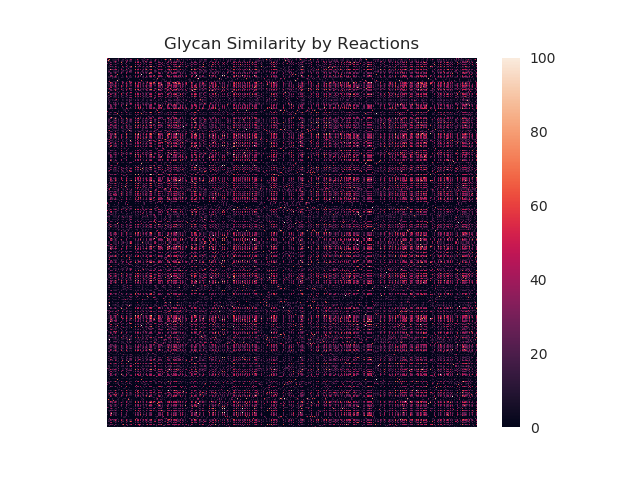
\includegraphics[scale=1.0]{images/heatmap_set_method.png} 
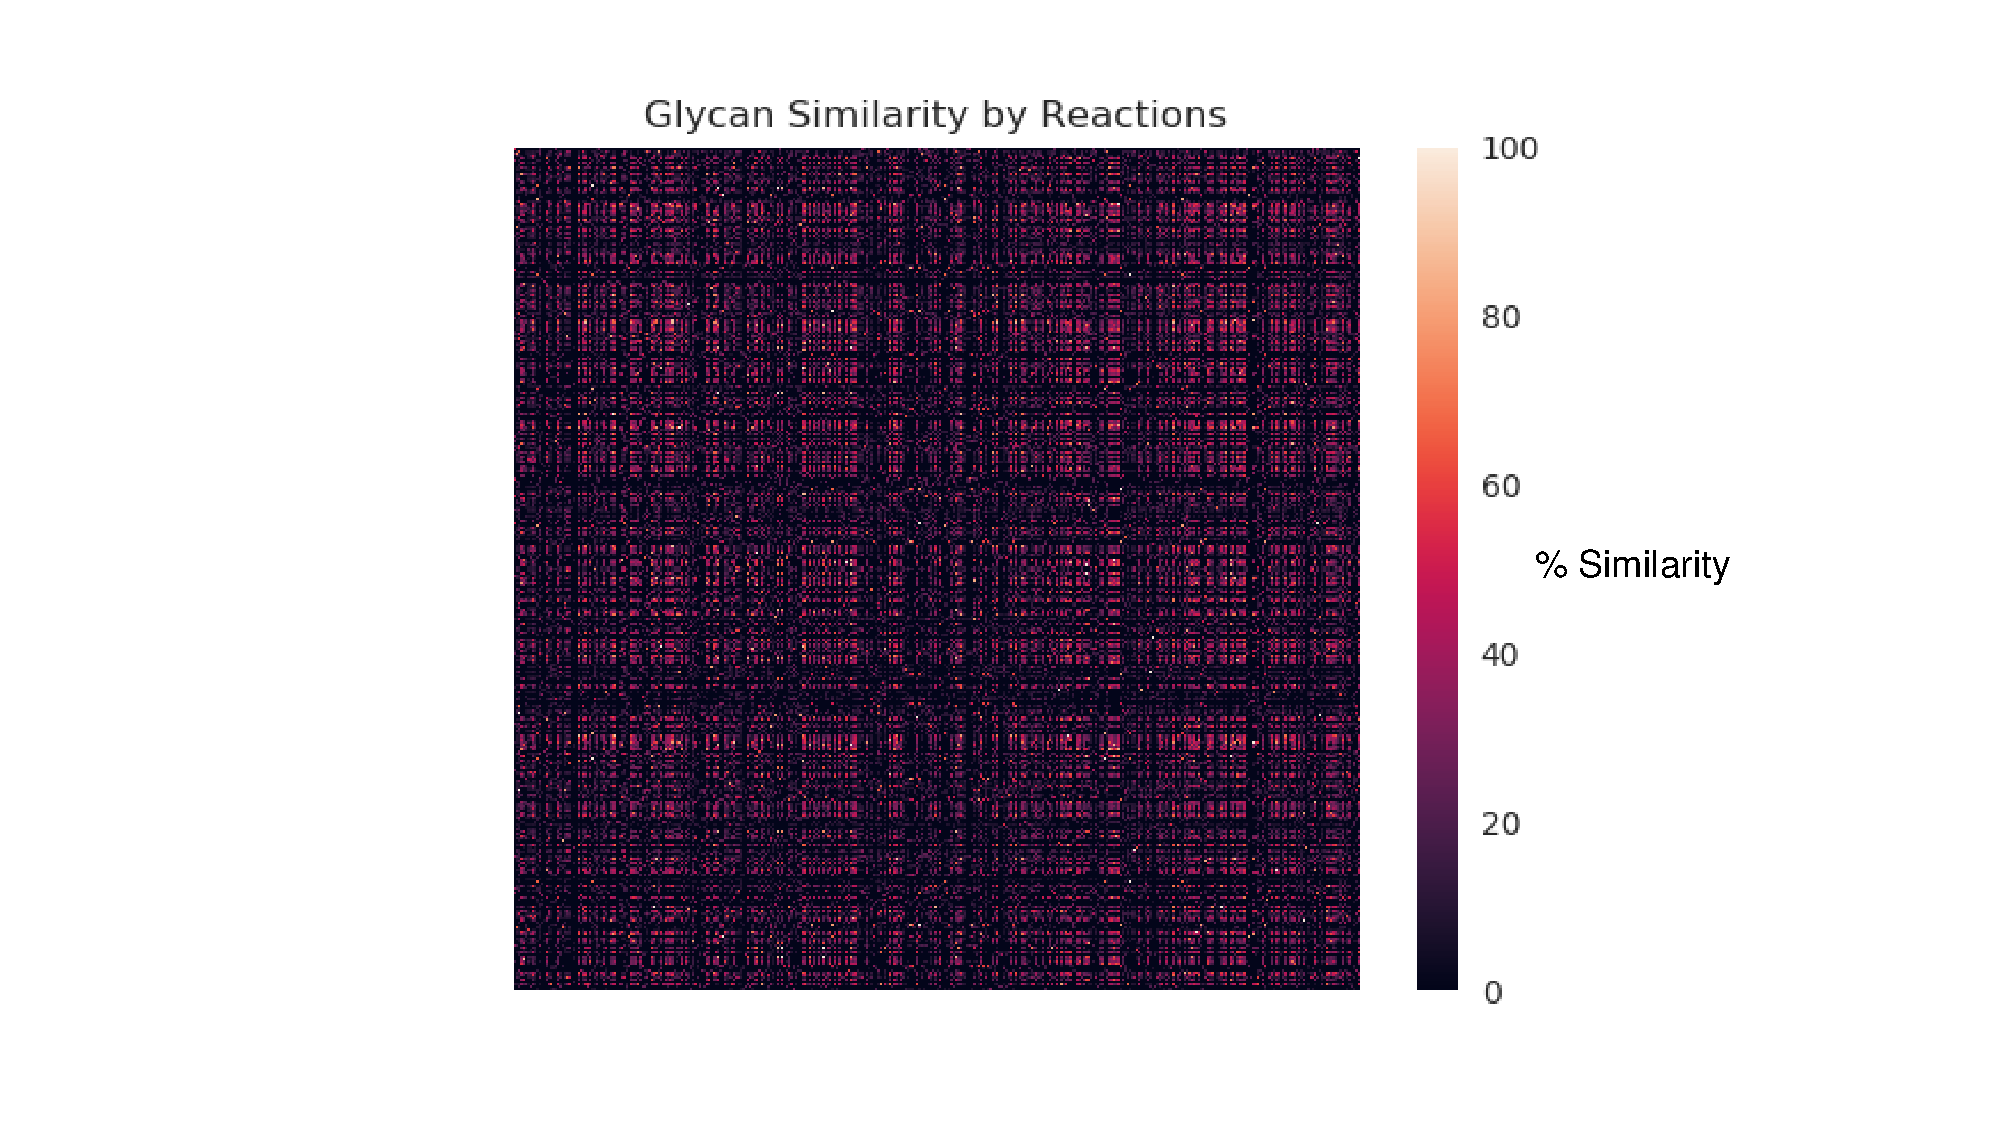
\includegraphics[scale=0.5]{images/heatmap_set_method.pdf} 
\caption{REMOVE THIS??? Glycan Reaction Sets Heatmap CROP IMAGE. Each axis is a list of Glycans IDs, not shown here because there are too many to display.}
\label{fig:heatmap_set_method}
\end{figure}

\subsection{Glycan Network Creation}
\label{sec:network_creation}

The binary adjacency matrix created in the previous step enables us to form a network, or undirected graph, representing glycan similarity, in which each of our glycans is a node and two nodes are joined by an edge if their glycans are marked as similar in the adjacency matrix. We use the Python package NetworkX \citep{hagberg2008exploring} for this purpose.

In our Python script \texttt{glycan\_reaction\_distances\_to\_network.py} we create a graph using the \texttt{from\_pandas\_adjacency} function from the NetworkX package. For the purposes of visualising this graph, we also need to assign each node to a point in the two-dimensional Euclidean plane. NetworkX provides several node positioning algorithms for this purpose, each of which takes a different approach to laying out the nodes in two-dimensional space according to various network metrics. The choice of any particular algorithm here does not altar the network topology, but can subjectively result in more or less informative graph visualisations. We choose the Fruchterman-Reingold force-directed algorithm \citep{fruchterman1991graph}.

We would like some method of judging if the relationships present in our network do indeed correlate with glycan similarity. From our original data query (see Section \ref{sec:glycan_databases}), we know which motifs are present in each glycan structure (according to the annotations in the GlyTouCan database). In the Python script \texttt{display\_network.py} we use this information to colour each node according to the set of motifs its glycan contains, and accordingly we would hope to see nodes of equal colour appearing in obvious clusters or communities in our graph.

In Section \ref{sec:distance_calc_set} we described two alternative methods of measuring similarity between glycans -- the Jaccard similarity coefficient applied to a glycan's reaction set, and the modified version applied to its reaction list (i.e. including reaction quantities). We asses the relative merits of these two methods via the \texttt{attribute\_assortativity\_coefficient} function in NetworkX, after setting a `motif' attribute for each node, whose value is the list of motifs which that glycan contains. The assortativity coefficient measures the similarity of connections in the graph with respect to a given attribute \citep{newman2003mixing}. However, the two graphs resulting from the two methods will almost certainly contain an unequal number of edges. In order to make the comparison fair, when creating the graph for the second method, rather than using the adjacency matrix, we use the similarity matrix (i.e. before thresholding has been applied) and the NetworkX function \texttt{from\_numpy\_array}, applying the similarity coefficients as edge weights. We then restrict our graph to only the $X$ highest weight edges, where $X$ is the number of edges found in the graph created using the first method, thus ensuring that both graphs have an equal number of edges.

Given the amount of glycans in our dataset, the resulting graph is large, and therefore can be uninformative when visualised as a whole. We are particularly interested in discovering groups of glycans deemed to be similar to each other, and so we use the \texttt{connected\_components} function in NetworkX to obtain lists of nodes which are connected to each other. Ordering these lists according to the number of nodes they contain allows us to select and visualise only the largest groups of connected components found in our graph. 

\subsection{Hierarchical Clustering}
\label{sec:clustering}

When plotted on a computer, the graphs described above can be explored by zooming in to focus on particular groups of nodes/glycans, potentially revealing interesting relationships between (for example) glycans sharing the same or similar motifs. The method though is dependent upon choosing a threshold value at which to make the binary choice between similar or dissimilar for any two glycans. An alternative method of clustering, avoiding this limitation, is the Unweighted Pair Group Method with Arithmetic Mean (UPGMA) \citep{gronau2007optimal}. This algorithm represents the structure of a pairwise similarity matrix as a rooted dendogram. The algorithm proceeds in s step-wise manner, calculating the average of the distances between all elements in two clusters $A$ and $B$. At the first step, each individual element (glycan, in our case) of the similarity matrix forms an individual cluster. The most similar clusters in any step are combined to form a new cluster, and the process is repeated until all clusters have been paired. The Python script \texttt{upgma\_glycans.py} creates one of these trees using the \texttt{DistanceTreeConstructor.upgma} function from the BioPython package.

The resulting tree is given in the form of an XML file, specifically phyloXML\footnote{\url{http://www.phyloxml.org}}. In order to aid visualisation, in our script \texttt{colour\_tree\_by\_motif\_group.py} we apply colour labels to all terminal nodes according to the motif sets belonging to the glycan represented by each node. We then traverse the tree from the terminal nodes upwards, applying the same colour labels if and only if the two children of a parent node have been labelled with the same colour. This provides a useful at-a-glance mechanism of identify clades of glycans sharing motif groups.

Finally, we use the phylogenetic tree visualisation software Archeopteryx\footnote{\url{https://sites.google.com/site/cmzmasek/home/software/archaeopteryx}} to visualise and explore the tree.


% \subsection{Blank}

% \subsubsection{Application Startup}
% \label{sec:startup}
% To use code--style text in-line, use \texttt{msc\_site}, or to apply to a section, use:

% \begin{verbatim}
% python manage.py runserver
% \end{verbatim}

% Another list example:

% \begin{enumerate}
% \item {\bf ProteinDomain} has attributes \texttt{name} and \texttt{pfam\_accession}.
% \item {\bf NodeVisualizationJsCode} The javascript library blah blah.
% \end{enumerate}

% \subsubsection{Singlespace Verbatim}
% \label{sec:template_tags}
% Like this:
% \singlespace
% \begin{figure}[H]
% \begin{verbatim}
% 
% 
%     
%         <ul>
%         ...
%         </ul>
%     
% 
% \end{verbatim}
% \caption{Example use of a custom Django filter in a template html file}
% \label{fig:custom_filter_code}
% \end{figure}
% \doublespace

\newpage
\section{Results}
\label{sec:results}

Possibly the most effective way to explore the landscape of glycan structure using the techniques described above in Section \ref{sec:method}, is to manipulate them in real-time on a computer, where it is possible to zoom in to examine regions of interest and to (in the case of the Archeopteryx tree viewer ) re-draw the tree in a multitude of different ways. In this section we present a selection of static images as we explore the glycan network and tree, illustrating both the validity of the techniques and some of the insights into glycan structure they provide.

% (Discuss them as you present them)\\

% - Walk through the network\\
% -- Figs 5 to 10: Glycan (un)connected components\\

% \begin{figure}[H]
% \centering 
% 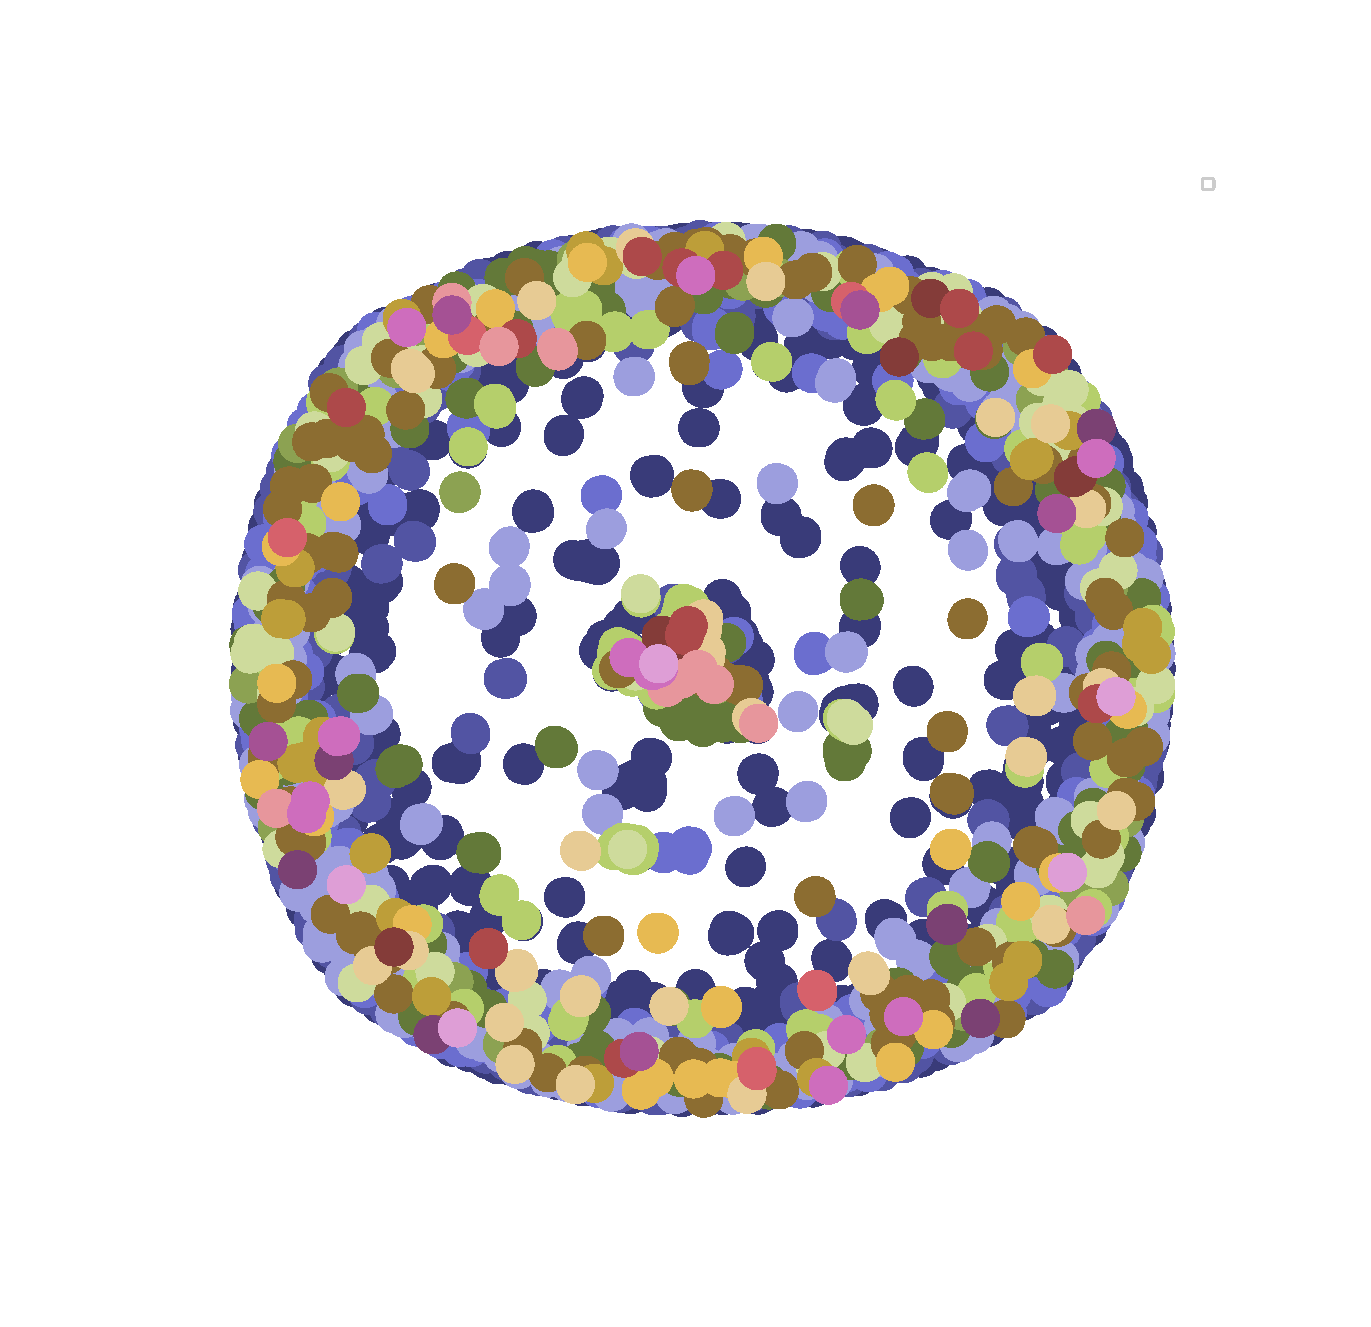
\includegraphics[scale=0.5]{threshold_87_conn_comp_1_method_set/threshold_87_full_network_method_set.eps} 
% \caption{Full network of glycans, with similarity determined using the reaction set method. CROP.}
% \label{fig:threshold_87_full_network_method_set}
% \end{figure}

\subsection{Glycan Network}
\label{sec:glycan_network}

Figures \ref{fig:threshold_87_conn_comp_1_method_set} through to \ref{fig:Neo_Lactosamine_vs_LacDiNAc} below were all produced using the reaction set method (see Section \ref{sec:distance_calc_set}). Figure \ref{fig:threshold_87_conn_comp_1_method_set} shows the most connected component of the network, with nodes (representing glycans) coloured according to the sets of motifs they contain. The figure legend details the colours assigned to each motif set. It is immediately apparent that, as hoped for, similarly coloured nodes exist in distinct communities, with mutual connections and often in close proximity, indicating high numbers of connections between glycans sharing the same motif sets. The fact that individual nodes of the same colour are still spatially separate indicates that despite sharing the same motifs, there are nevertheless structural differences between those glycans -- this is exactly as we would expect, given that all glycans taken from the database are structurally distinct, albeit many show similarity in terms of their motifs. In order to examine the relationships between these groups more closely, we need to zoom in and inspect the network in more detail.

\begin{sidewaysfigure}
\centering 
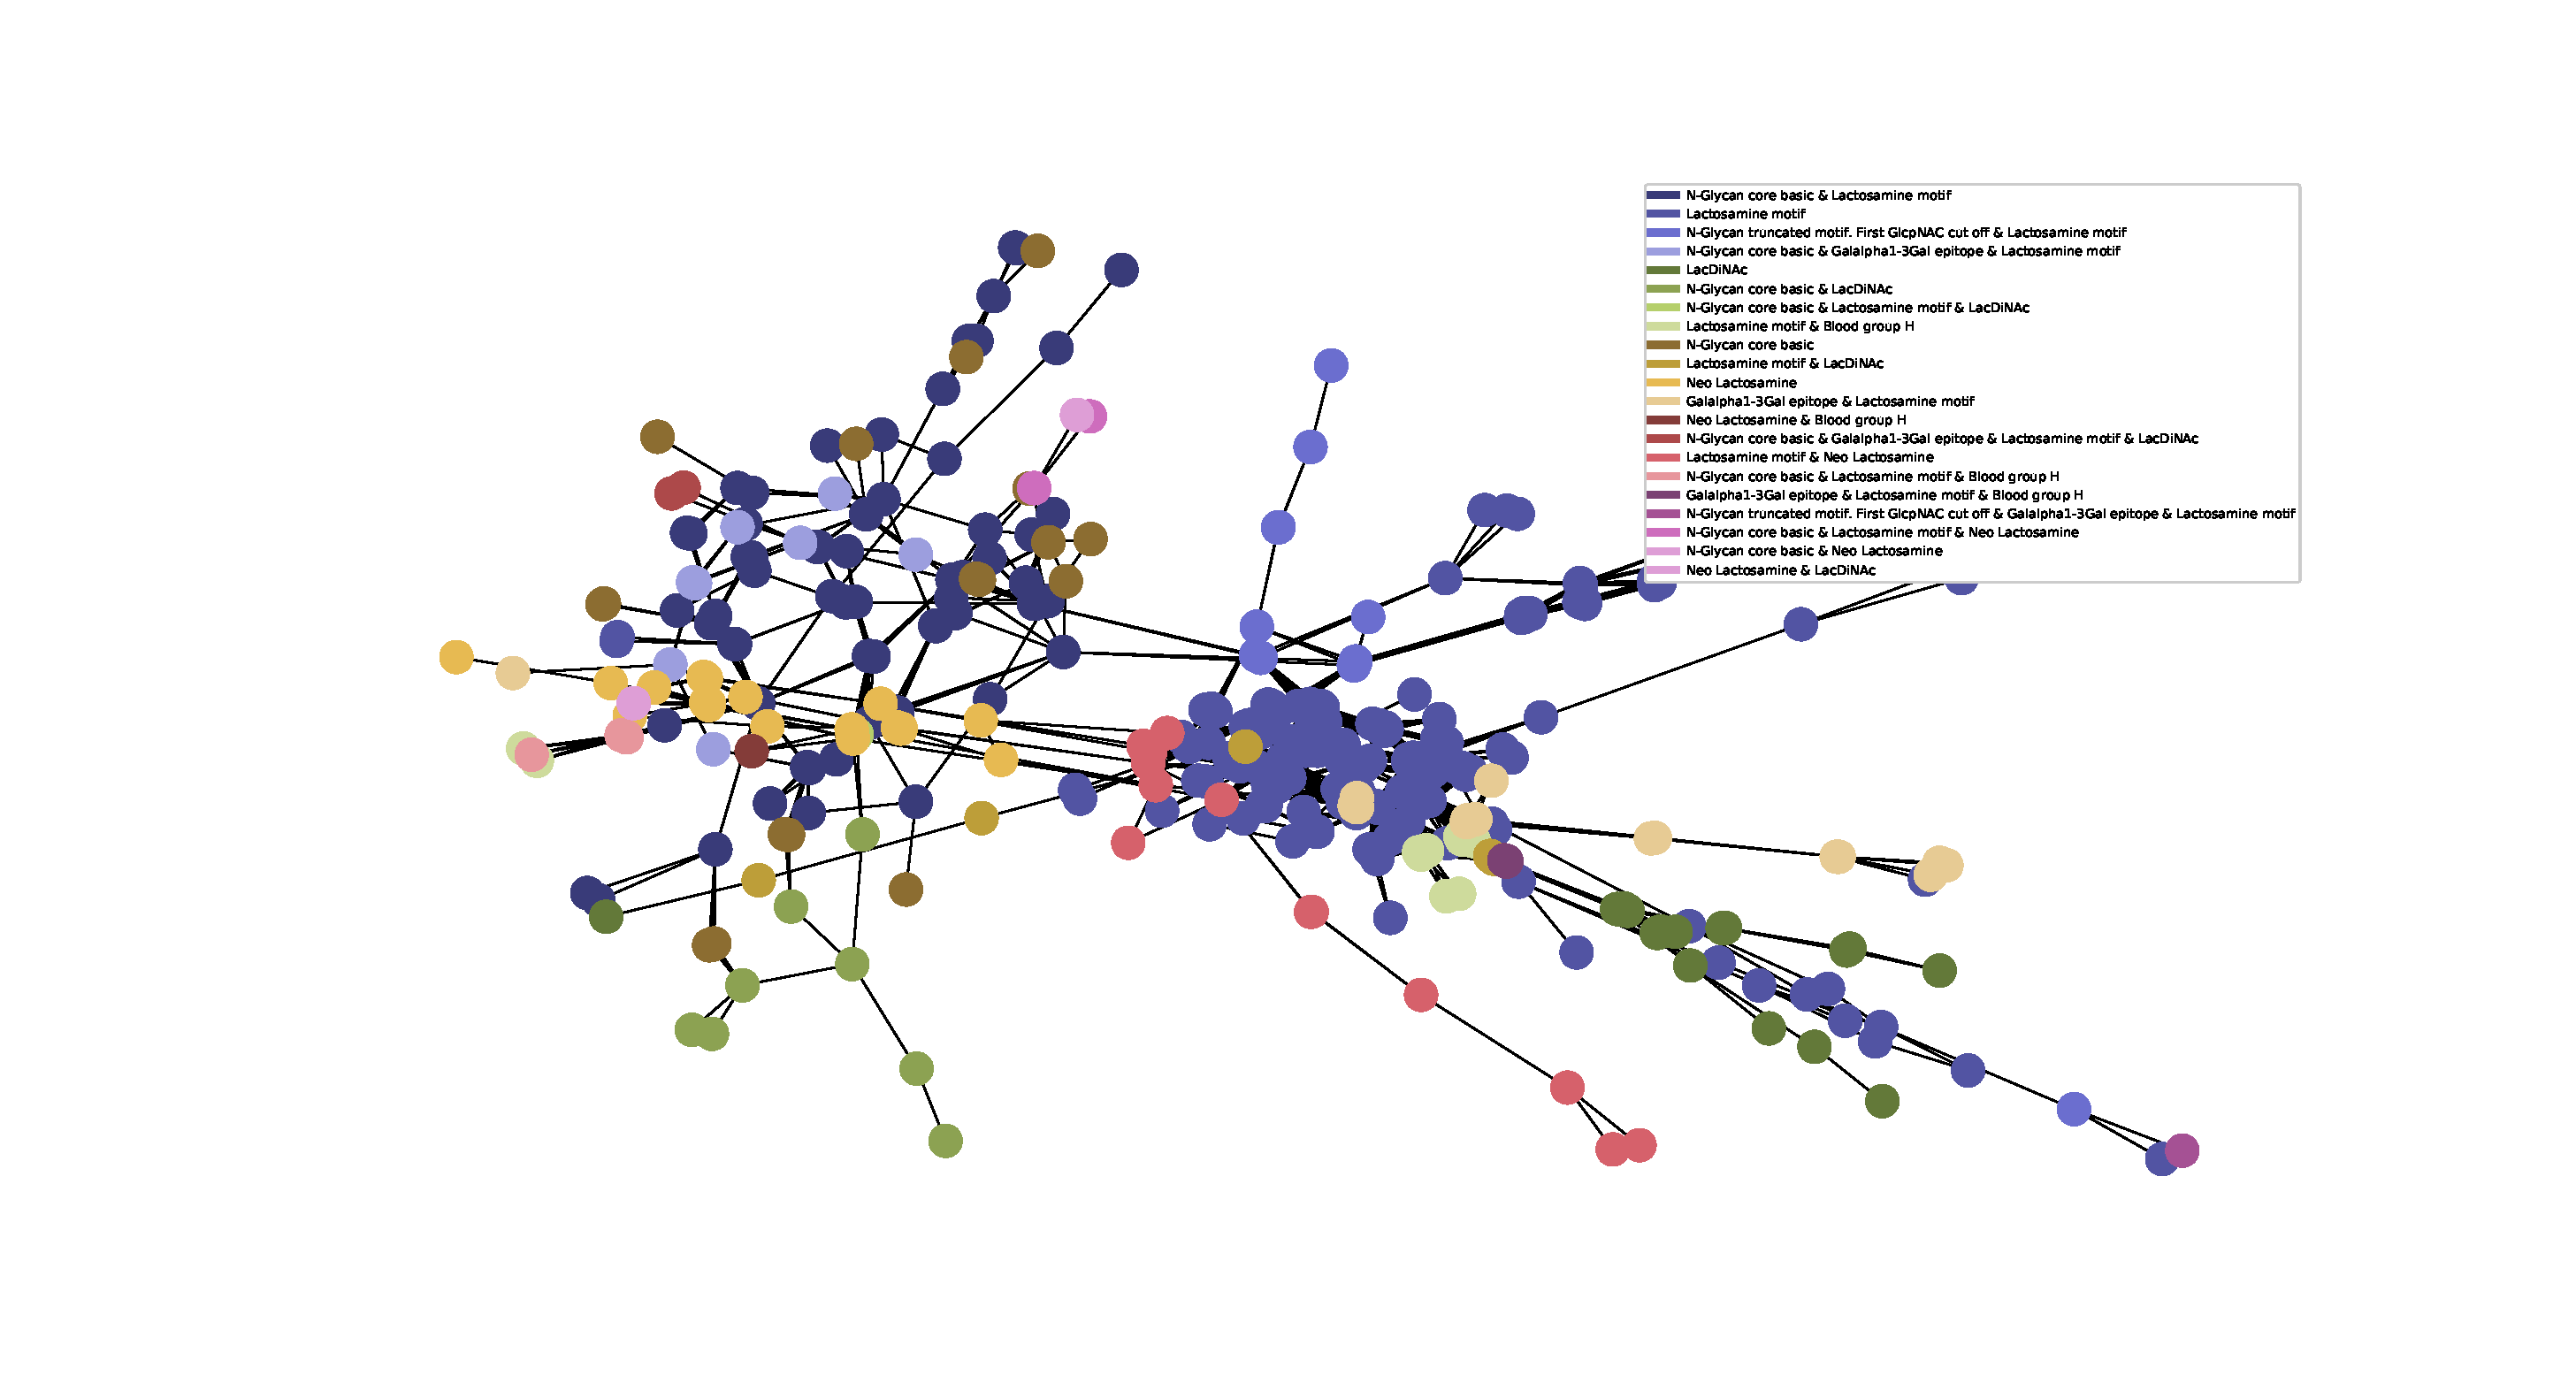
\includegraphics[scale=0.5]{threshold_87_conn_comp_1_method_set/threshold_87_conn_comp_1_method_set.eps} 
\caption{Most connected component of a network of glycans, with similarity determined using the reaction set method. CROP.}
\label{fig:threshold_87_conn_comp_1_method_set}
\end{sidewaysfigure}
\clearpage

\begin{figure}[H]
\centering 
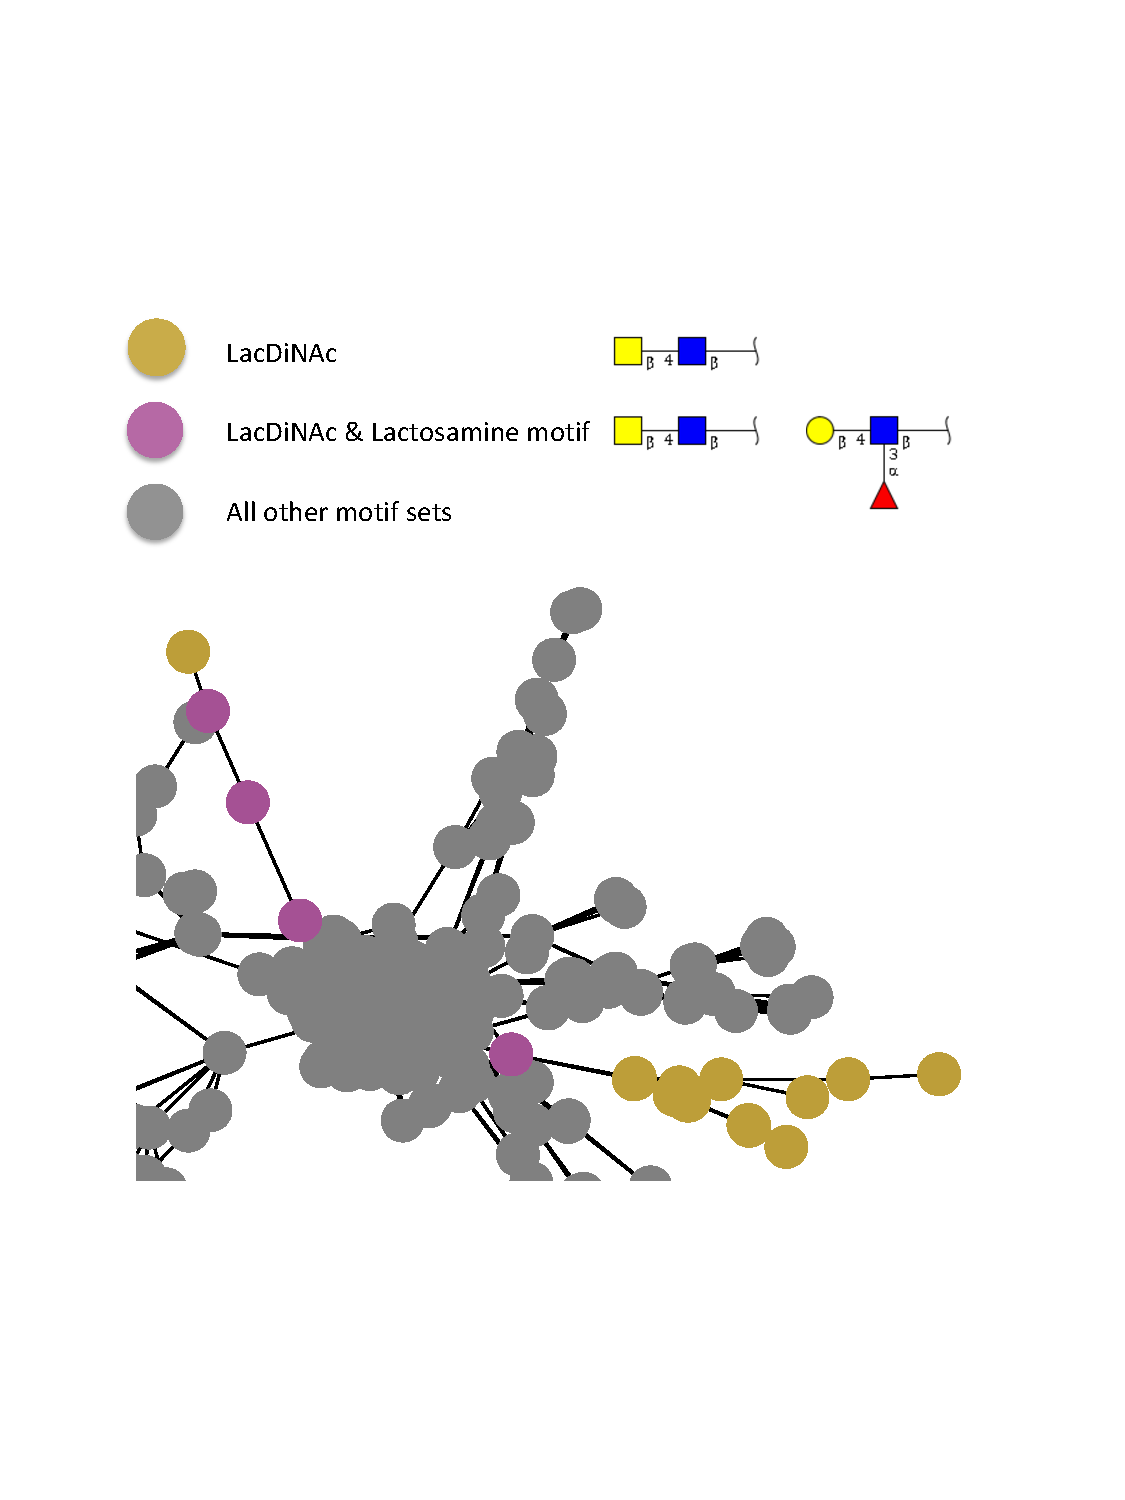
\includegraphics[scale=0.9]{motif_similarity_exploration/LacDiNAc_vs_Lactosamine_motif_LacDiNAc.pdf} 
\caption{Glycans containing the LacDiNAc motif (orange nodes) are connected solely to glycans containing the LacDiNAc and Lactosamine motifs (purple nodes).}
\label{fig:LacDiNAc_vs_Lactosamine motif,LacDiNAc}
\end{figure}

In Figure \ref{fig:LacDiNAc_vs_Lactosamine motif,LacDiNAc}, we highlight only two groups of glycans -- those containing the single motif LacDiNAc (coloured orange), and those containing two motifs -- LacDiNAc and the Lactosamine motif (coloured purple). All other glycans are coloured grey. In the same figure, we also display the glycan motifs. The two motif sets are similar to each other in two respects -- firstly, they both share exactly the same motif, LacDiNAc, and secondly, Lactosamine and LacDiNAc have in common a $\beta$ anomeric N-Acetyl-D-Glucosamine monosaccharide (the blue square). It is reasonable then to assume that glycans containing either of these motif sets would be structurally similar, and indeed the figure illustrates that the glycans in our network with just the LacDiNAc motif  (orange) are solely connected either to each other or to glycans containing the LacDiNAc and Lactosamine motifs.

Another example is shown in Figure \ref{fig:Galalpha1-3Gal_epitope_Lactosamine_motif_Blood_group_H_vs_Lactosamine_motif_Blood_group_H}, this time highlighting glycans containing the Galalpha1-3Gal epitope, Lactosamine, and Blood group H motifs (orange), and those containing Lactosamine, and Blood group H motifs (green). Direct connections exist between the two groups, as we would expect given that one group contains two out of the three motifs present in the other.

\begin{figure}[H]
\centering 
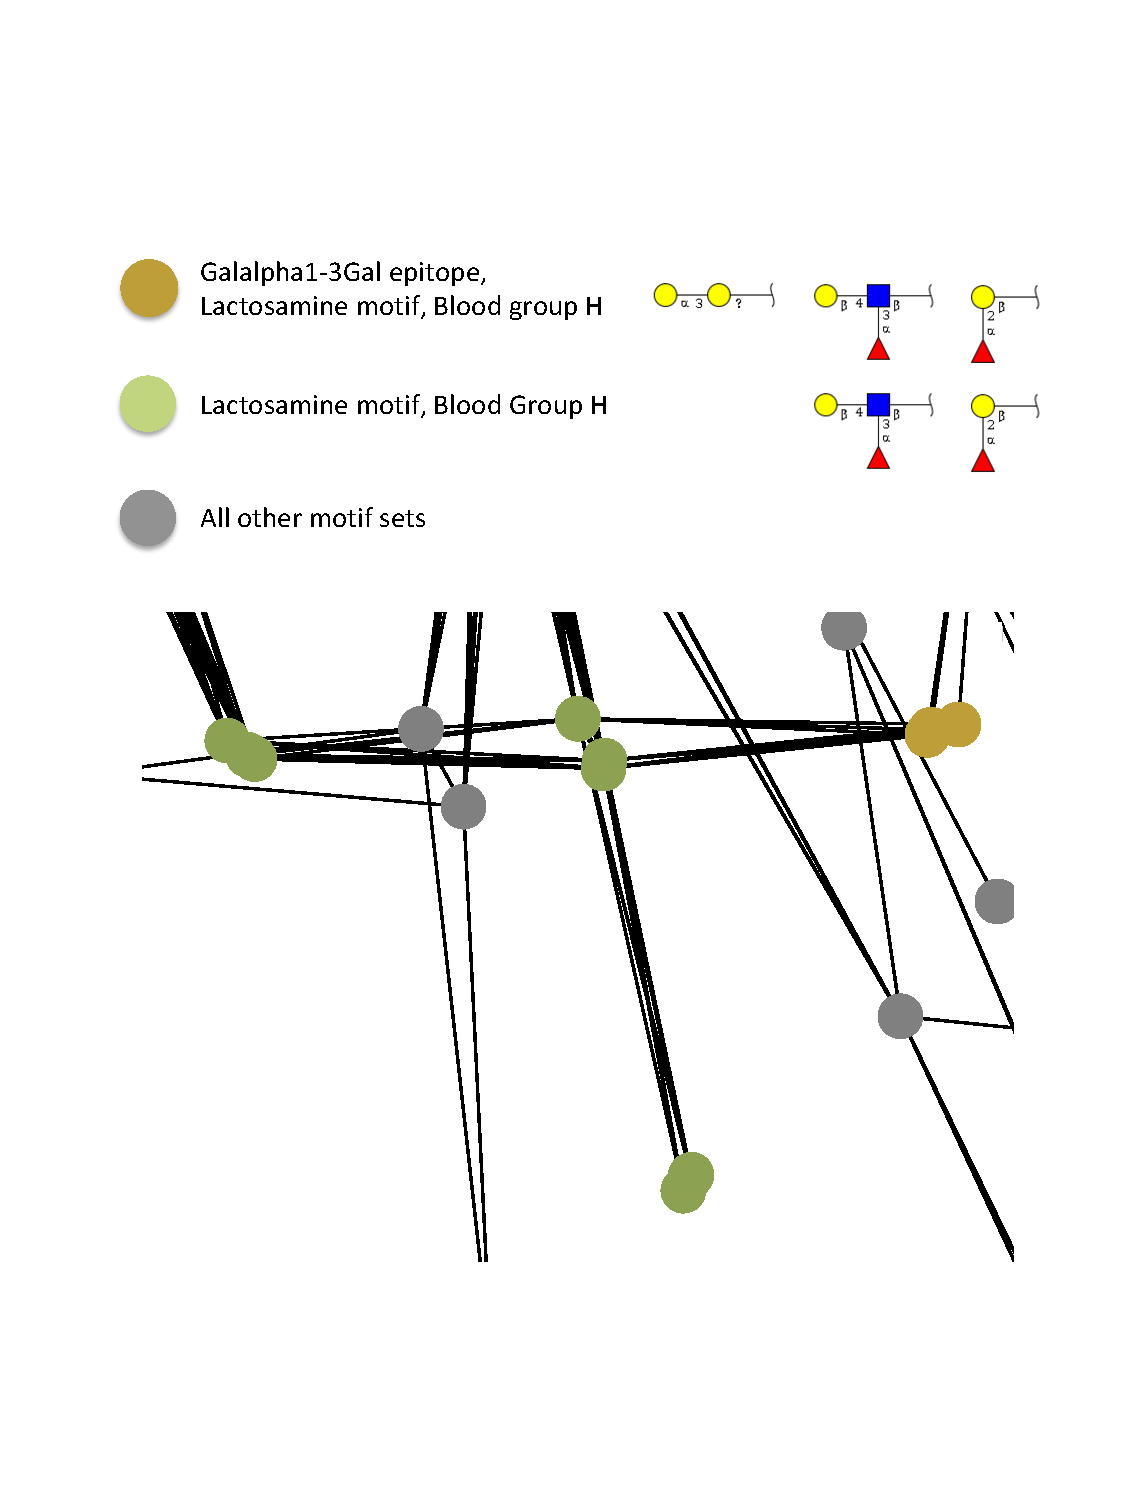
\includegraphics[scale=0.85]{motif_similarity_exploration/Galalpha1-3Gal_epitope__Lactosamine_motif__Blood_group_H_vs_Lactosamine_motif__Blood_group_H.pdf} 
\caption{Glycans containing the Galalpha1-3Gal epitope, Lactosamine, and Blood group H motifs (orange nodes) are connected to glycans containing the Lactosamine, and Blood group H motifs (green nodes).}
\label{fig:Galalpha1-3Gal_epitope_Lactosamine_motif_Blood_group_H_vs_Lactosamine_motif_Blood_group_H}
\end{figure}

Conversely, in each of Figures \ref{fig:N-Glycan_core_basic_vs_Lactosamine_motif} and \ref{fig:Neo_Lactosamine_vs_LacDiNAc}, we highlight two groups of glycans which do not share similar motifs. In these instances, there are no direct connections between the two glycan groups, implying significant structural differences, as we would expect given the differences in motifs. Network graphs created using the reactions list method, as opposed to the reactions set method, exhibit the same types of relationships and we omit them here.

\begin{figure}[H]
\centering 
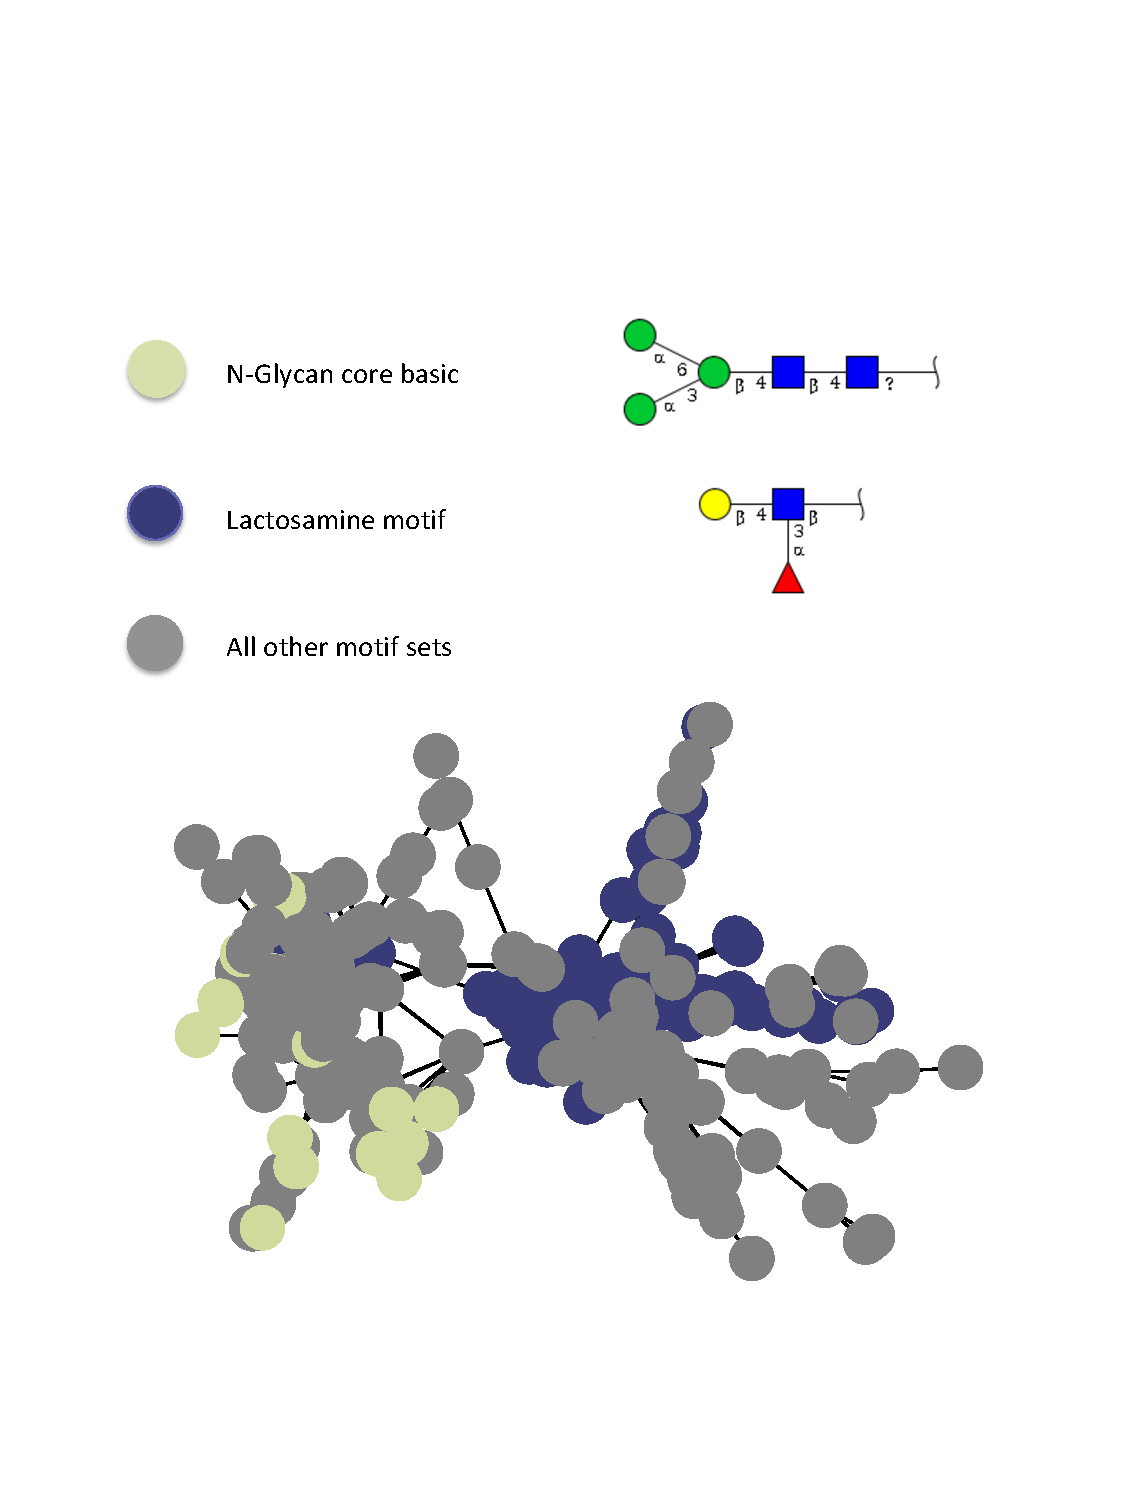
\includegraphics[scale=0.9]{motif_similarity_exploration/N-Glycan_core_basic_vs_Lactosamine_motif.pdf} 
\caption{Glycans containing the N-Glycan core basic motif (green nodes) are not directly connected to glycans containing the Lactosamine motif (blue nodes).}
\label{fig:N-Glycan_core_basic_vs_Lactosamine_motif}
\end{figure}

\begin{figure}[H]
\centering 
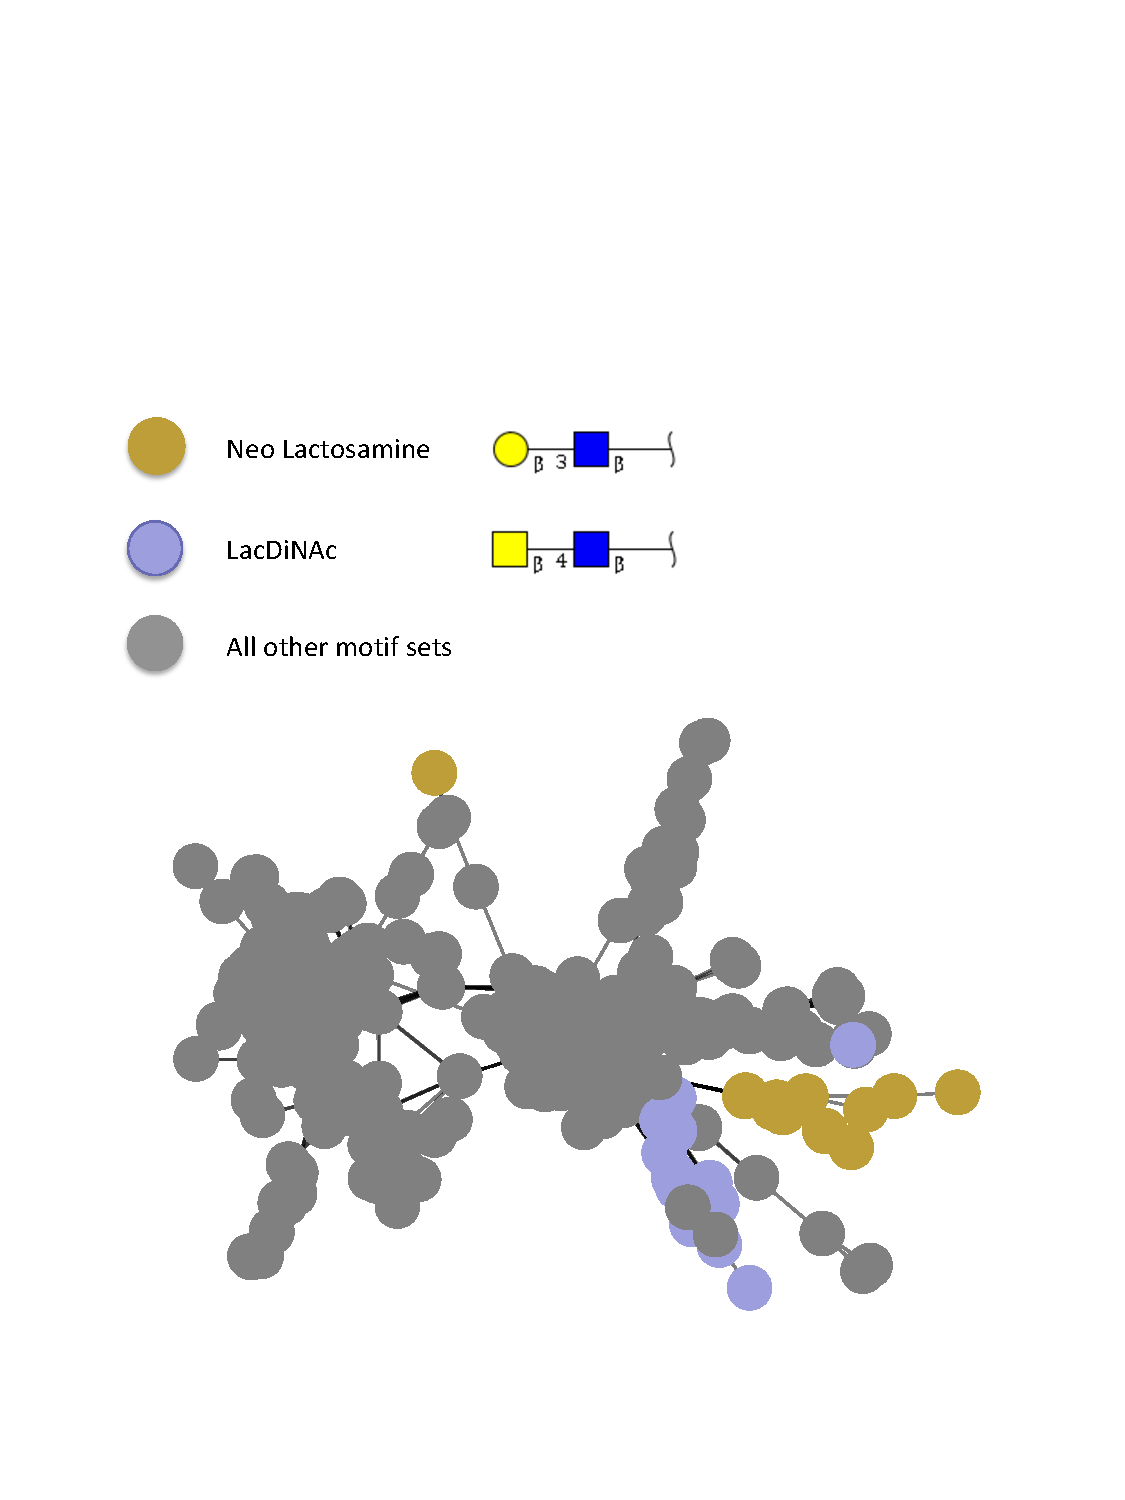
\includegraphics[scale=0.9]{motif_similarity_exploration/Neo_Lactosamine_vs_LacDiNAc.pdf} 
\caption{Glycans containing the Neo Lactosamine motif (orange nodes) are not directly connected to glycans containing the LacDiNAc motif (violet nodes).}
\label{fig:Neo_Lactosamine_vs_LacDiNAc}
\end{figure}

\newpage
\subsection{Assortativity Coefficient}
\label{sec:assortativity_coefficient}

The assortativity coefficients calculated for the two alternative similarity measures are:\\

Reaction set method: {\bf 0.93}\\
\indent Reaction list method {\bf 0.97}\\

The higher value for the reaction list method suggests that there is a benefit to taking into account reaction quantities, rather than just presence, when measuring glycan similarity.

\subsection{UPGMA Hierarchical Clustering}
\label{sec:clustering_results}

Figure \ref{fig:full_tree_zoomed} shows a magnified section of the full tree (in cladogram form) produced using UPGMA hierarchical clustering, applied to the distance matrix obtained using the reaction list method. The terminal nodes, which represent individual glycans, are labelled with both the names of the motifs present in each glycan, and, in brackets, the glycan ID (as taken from the GlyTouCan database). The visualisation software dynamically adjusts the number of terminal nodes for which it displays labels in order to avoid clutter. We can see via the terminal labels and the branch colours that there are distinct clades of glycans which share the same motif sets, providing further evidence of the suitability of our method for determining glycan similarity. Furthermore, adjacent clades of different colours often have motifs in common, analogous to the connected nodes we observed in the glycan network.

\begin{sidewaysfigure}
\centering 
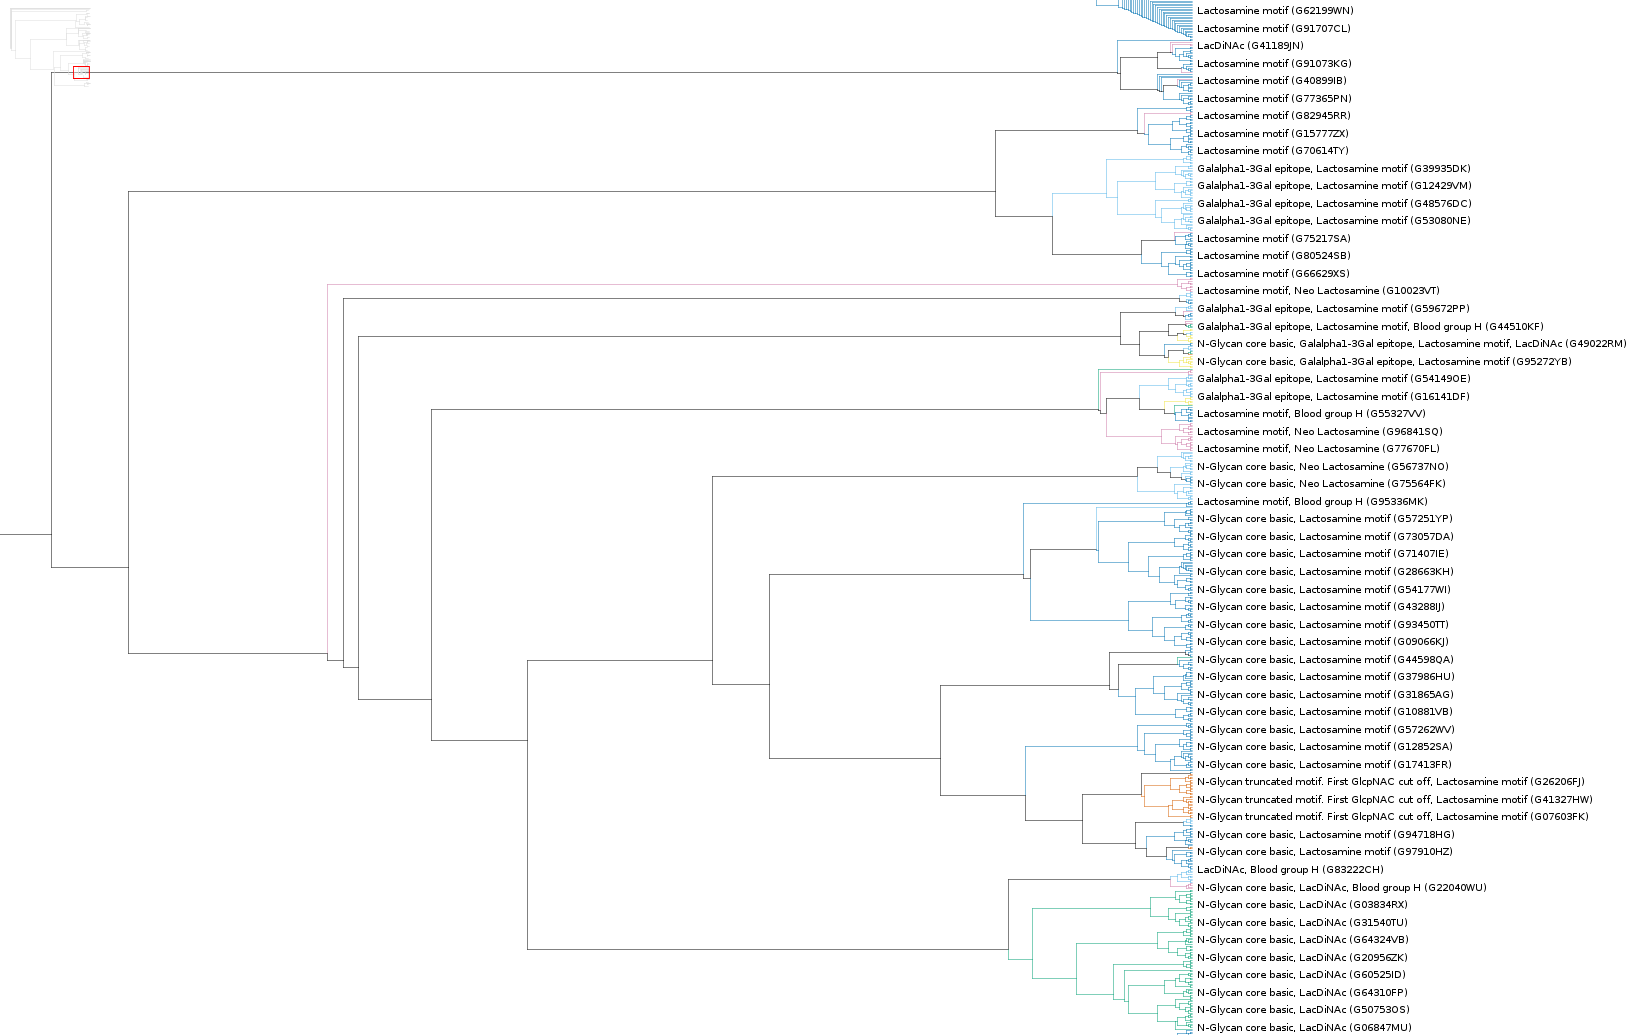
\includegraphics[scale=0.3]{trees/zoomed_full_tree_cladogram.png} 
\caption{Full depth UPGMA tree (zoomed in to subsection). Clades of equal colour indicate clusters of glycans sharing the same motifs sets.}
\label{fig:full_tree_zoomed}
\end{sidewaysfigure}
\clearpage

subsubsection{Motif Discovery}
A detailed inspection of the UPGMA tree reveals some features which, initially, seem to be at odds with the notion of shared motifs between simlar glycans observed so far. For example, in Figure \ref{fig:full_tree_LacDiNAc}, a glycan with the sole motif LacDiNAc (highlighted in red) appears amongst a cluster of glycans containing only the `N-Glycan truncated motif first GlcpNAC cut off' motif. However, looking up the structure of this glycan in the GlyTouCan database reveals that this glycan does in fact contain the `N-Glycan truncated motif first GlcpNAC cut off' motif as well as LacDiNAc, it just has not been annotated as containing it. Figure \ref{fig:rogue_lacdinac_a} shows the full glycan structure, Figure \ref{fig:rogue_lacdinac_b} shows the LacDiNAc motif, with which the glycan has been correctly annotated, and Figure \ref{fig:rogue_lacdinac_c} shows the `N-Glycan truncated motif first GlcpNAC cut off' motif which the glycan has not been annotated as containing, but which is clearly seen in the full structure (Figure \ref{fig:rogue_lacdinac_a}).

--- Fig 12: zoomed-in tree\\
-- describe the clades, relate them to the network if poss\\
--- therefore make a comparison between jaccard + network and UPGMA tree methods\\
---- Are there similarities between tree and network? (network is only a vis tool, the tree is the real deal) \\

\begin{sidewaysfigure}
\centering 
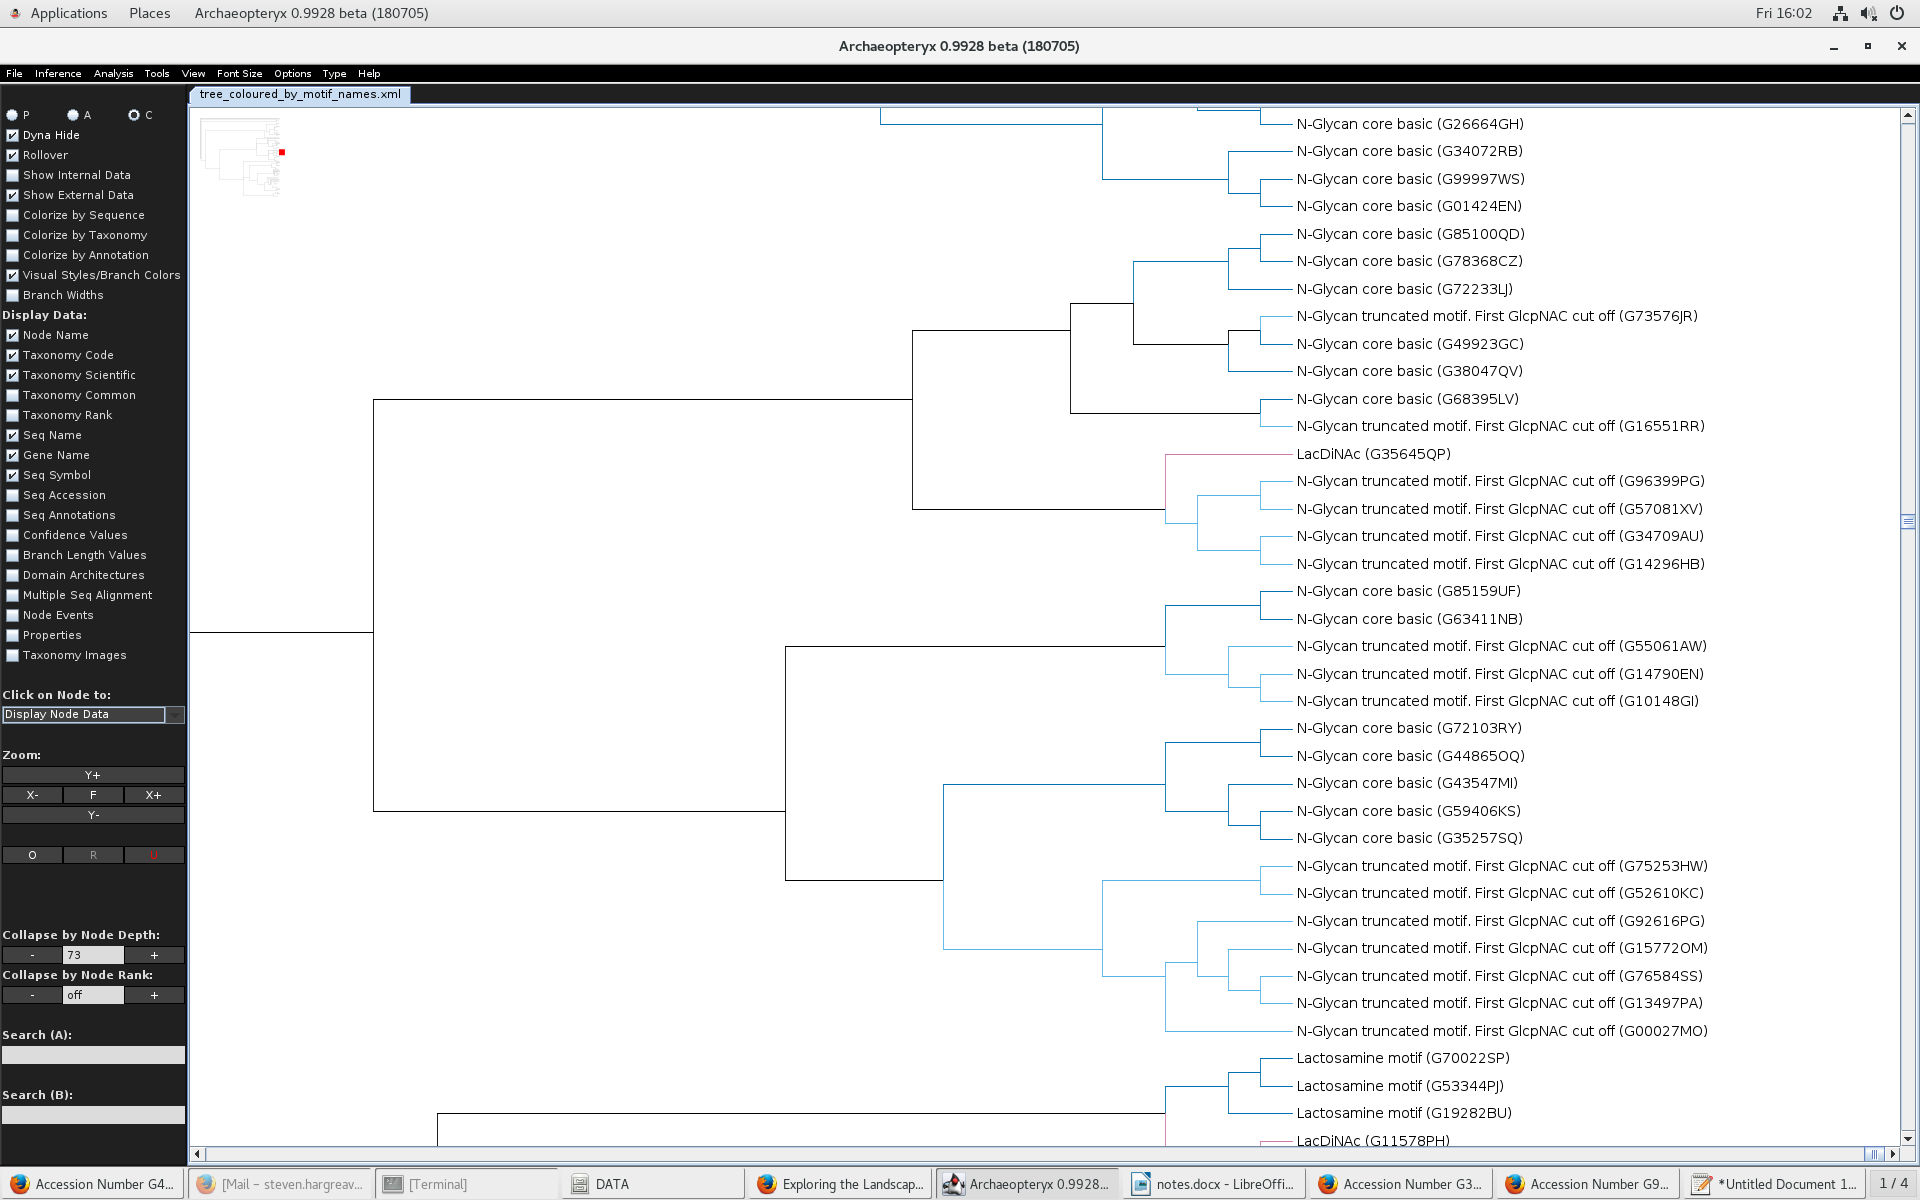
\includegraphics[scale=0.3]{trees/rogue_LacDiNAc_in_tree.png} 
\caption{A glycan (highlighted in red) which has a missing motif annotation in the GlyTouCan database has been correctly clustered with glycans sharing the same motif.}
\label{fig:full_tree_LacDiNAc}
\end{sidewaysfigure}
\clearpage

\begin{figure*}[ht!]
    \centering
    \begin{subfigure}[t]{1.0\textwidth}
        \centering
        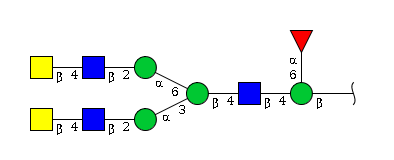
\includegraphics[scale=0.6]{trees/rogue_LacDiNAc_structure.png}
        \caption{Actual structure of the glycan highlighted in red in Figure \ref{fig:full_tree_LacDiNAc}.}
        \label{fig:rogue_lacdinac_a}
    \end{subfigure}%
    \\
    \bigbreak
    ~ 
	\\
    \begin{subfigure}[t]{1.0\textwidth}
        \centering
        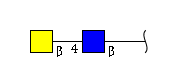
\includegraphics[scale=0.6]{trees/LacDiNAc_motif.png}
        \caption{Correctly annotated LacDiNAc motif.}
        \label{fig:rogue_lacdinac_b}
    \end{subfigure}
    \\
    \bigbreak
    ~ 
	\\
    \begin{subfigure}[t]{1.0\textwidth}
        \centering
        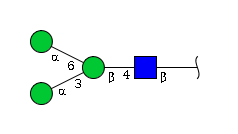
\includegraphics[scale=0.6]{trees/N-Glycan_truncated_motif__First_GlcpNAC_cut_off_motif.png}
        \caption{Missing motif annotation `N-Glycan truncated motif First GlcpNAC cut off'}
        \label{fig:rogue_lacdinac_c}
    \end{subfigure}
    \caption{The actual structure of the glycan highlighted in red in Figure \ref{fig:full_tree_LacDiNAc} and its present and missing motif annotations.}
\label{fig:rogue_lacdinac}
\end{figure*}


\newpage
\section{Discussion}
\label{sec:discussion}
(On the bigger picture)\\
Should have calculated statistical significance of assortativity coeffs. Could use bootstrap etc.\\

Uncertainties in the glycan db (carbon numbers, no. of links etc.) (what proportion? 33000/100000) limit our coverage, as do computing resources (RAM, CPU).\\

We're dependent upon the coverage and quality of glycan databases, and glycan formats (new ones keep appearing so WURCS 2.0 could be out-of-date soon? the field is in its infancy compared to e.g. protein structure prediction - give some example dates) although this technique can actually help with annotation (e.g. detecting missing motifs).\\

For networks, threshold and layout choice is key and a manual process\\


\newpage
\section{Further Work}
\label{sec:further_work}

Can use more advanced SPARQL query to get reaction breakdown (so should increase both number of glycans and accuracy)\\

Deal with uncertainties in DB.\\
But we can use some of the certain reactions from the uncertain structures to increase our coverage\\

Perform on better machines to increase glycan coverage (i.e. eliminate filtering step)\\

try bi-clustering on the original jaccard matrix (will need to include ALL reactions for each pairwise comparison, rather than just those present in the two glycans under consideration as I presently do). See John's email 17th July for method details.\\

(tree) Kernel methods (see “Glycan classification with tree kernels” (Yoshihiro Yamanishi, Francis Bach and Jean-Philippe Vert) \\

- New dataset, samples by cell / tissue\\
- details on what we would do
-- Work already done (web scraping for data)\\
-- Format conversion problems\\
--- conversion software breaks for linearcode to WURCS (can't handle uncertainties)\\

Compare full structures, not just reactions\\

Compare sets of structures\\

Use neighbour joining or K-means instead of UPGMA (can you say why that might be useful?)\\

Other glycan databases?\\

KEGG?\\

Use LGL, organic cytoscape for vis\\

chi-squared to compare two (quantified) reaction profiles\\

\citep{porter2009motif} provides some `rules' on incompatibilities (Table 1) and (??? graphs) which we could compare our results with\\

could try an alternative version of clustering, as used for Fig 4 D of "A motif-based analysis of glycan array data to determine the specificities of glycan-binding proteins", for comparison with my version\\

\newpage
\section{Conclusions}
\label{sec:conclusions}

we've demonstrated encouraging results without needing to perform complex tree comparisons\\

\newpage
\bibliographystyle{agsm}
\bibliography{bibliography}


\newpage
\section*{Appendices}
\appendix
%\chapter{}
\section{Software Dependencies}
\label{sec:software_dependencies}
Table \ref{tab:software_dependencies} lists the packages necessary to run the python code used to produce the results described in this paper. The program code itself can be cloned into the current directory by typing the following command in a command window (assuming the Git\footnote{\url{https://git-scm.com/}} application is already installed):

\begin{verbatim}
git clone https://github.com/ImperialCollegeLondon/glycans.git
\end{verbatim}

\begin{table}[h]
\centering
%\resizebox{\columnwidth}{!}
\rowcolors{1}{}{lightblue}
\begin{tabular}{|c|c|} \hline
{\bf Package Name} & {\bf Version} \\ \hline
biopython   &               1.72 \\ \hline
fontconfig    &             2.12.6 \\ \hline
glypy       &               0.12.2 \\ \hline
html5lib   &                1.0.1 \\ \hline
httplib2   &                0.11.3 \\ \hline
matplotlib &                2.2.2 \\ \hline
networkx  &                 2.1 \\ \hline
numpy    &                  1.14.3 \\ \hline
numpy-base   &              1.14.5 \\ \hline
pandas  &                   0.23.2 \\ \hline
python   &                  3.6.6 \\ \hline
rdflib  &                   4.2.2 \\ \hline
scipy   &                   1.1.0 \\ \hline
seaborn  &                  0.8.1 \\ \hline
sparqlwrapper   &           1.8.0 \\ \hline
urllib3      &              1.23 \\ \hline
\end{tabular}
\caption{Python software packages necessary to run the program code associated with this project.}
\label{tab:software_dependencies}
\end{table}
\clearpage

%\chapter{}
\section{Glycan Databases and Structure Formats}
\label{sec:glycan_dbs_and_formats}
Table \ref{tab:glycan_databases} lists some glycan databases, the number of glycans they contain, and the glycan structure formats they provide.

\begin{table}[h]
\begin{minipage}{\textwidth}
\centering
%\resizebox{\columnwidth}{!}
\rowcolors{1}{}{lightblue}
\begin{tabular}{|c|c|p{7cm}|} \hline
{\bf Database Name} & {\bf No. glycans}  & {\bf Formats} \\ \hline
KEGG Glycan\footnote{\url{https://www.genome.jp/dbget-bin/www_bfind_sub?mode=bfind&max_hit=1000&locale=en&serv=gn&dbkey=glycan&keywords=*&page=1}} & 504 & KCF \\ \hline
GlyConnect\footnote{\url{https://glyconnect.expasy.org/browser/structures/2259}} & 3768 & IUPAC \\ \hline
UniCarbKB\footnote{\url{http://www.unicarbkb.org/}} & 3238 & note\footnote{Website not working at time of publication} \\ \hline
GlyTouCan\footnote{\url{https://glytoucan.org/}} & 105050 & WURCS, GlycoCT, IUPAC Condensed, IUPAC Extended \\ \hline
\end{tabular}
\caption{Glycan databases, and the structure formats they provide.}
\label{tab:glycan_databases}
\end{minipage}
\end{table}

\noindent Different glycan structure formats exist. The number of glycans in the GlyTouCan database for each format it supports are shown in Table \ref{tab:glycan_format_counts}.

\begin{table}[h]
\centering
\rowcolors{1}{}{lightblue}
\begin{tabular}{|c|c|c|} \hline
{\bf Format Name} & {\bf Number of Glycans} & {\bf Comments} \\ \hline
GlycoCT & 45438 & Verbose, no longer supported\\ \hline
IUPAC & 14517 & \\ \hline
IUPAC condensed & 73329 & \\ \hline
IUPAC extended & 73329 & \\ \hline
WURCS & 105050 & Most recently published \\ \hline
\end{tabular}
\caption{Glycan counts in the GlyTouCan database for different glycan structure formats.}
\label{tab:glycan_format_counts}
\end{table}

\singlespace
\noindent Additional glycan resources can be found at the following URLs:
\begin{itemize}
\item \path{https://biosciencedbc.jp/en/db-link/d09-dblink}
\item \path{http://www.functionalglycomics.org/static/consortium/links.shtml}
\item \path{https://biosciencedbc.jp/en/db-link/d09-dblink}
\end{itemize}
\doublespace
\clearpage

\section{SPARQL queries}
\label{sec:sparql_queries}
SPARQL queries may be run programmatically, or against the GlyTouCan database at the following `SPARQL Endpoint' (a web query interface):\\

\noindent \path{https://ts.glytoucan.org/sparql}\\

\noindent The following SPARQL query returns all Glycan IDs, WURCS format strings, and motif IDs. Results for glycans with multiple motifs will be spread across multiple lines:\\

\singlespace
\begin{verbatim}
  PREFIX glycan: <http://purl.jp/bio/12/glyco/glycan#>
  PREFIX glytoucan:  <http://www.glytoucan.org/glyco/owl/glytoucan#>

  SELECT DISTINCT ?Saccharide ?PrimaryId ?Sequence 
                  ?Motif ?MotifPrimaryId
  FROM <http://rdf.glytoucan.org/core>
  FROM <http://rdf.glytoucan.org/sequence/wurcs>
  FROM <http://rdf.glytoucan.org/motif>
  WHERE {
    ?Saccharide glytoucan:has_primary_id ?PrimaryId .
    ?Saccharide glycan:has_glycosequence ?GlycoSequence .
    ?GlycoSequence glycan:has_sequence ?Sequence .
    ?GlycoSequence glycan:in_carbohydrate_format 
      glycan:carbohydrate_format_wurcs.
    OPTIONAL { ?Saccharide glycan:has_motif ?Motif .
               ?Motif glytoucan:has_primary_id ?MotifPrimaryId } .
  }
  ORDER BY ?PrimaryId
\end{verbatim}
\doublespace

\newpage
\noindent This SPARQL query returns all Motif IDs and motif labels:\\

\singlespace
\begin{verbatim}
  PREFIX glycan: <http://purl.jp/bio/12/glyco/glycan#>
  PREFIX glytoucan:  <http://www.glytoucan.org/glyco/owl/glytoucan#>

  SELECT DISTINCT ?Motif ?MotifPrimaryId ?MotifLabel
  FROM <http://rdf.glytoucan.org/core>
  FROM <http://rdf.glytoucan.org/sequence/wurcs>
  FROM <http://rdf.glytoucan.org/motif>
  WHERE {
    ?Saccharide glycan:has_motif ?Motif .
    ?Motif glytoucan:has_primary_id ?MotifPrimaryId.
      ?Motif rdfs:label ?MotifLabel
  }
  ORDER BY ?MotifPrimaryId
\end{verbatim}
\doublespace


% \section{Example JavaScript Code}
% \label{sec:gains_js_code}
% JavaScript code for determining the width of a rectangle representing total domain gains for each node. The function \texttt{domian\_count} loops through all of the xml property tags associated with a node, parses their content, and returns a dictionary with domain names as keys, and their copy number as the values. The function \texttt{calc\_dom\_deltas} takes the domain count dictionaries of both a parent and a child node, and calculates the total gains and losses across all domains from the parent to the child. The in-line \texttt{function(n)} of the \texttt{nodeEnter} code is called by the underlying D3 library for every node in our data object (which has previously been created from a phyloXML file), and, using the two functions \texttt{domian\_count} and \texttt{calc\_dom\_deltas}, determines which numeric value to apply to the `width' attribute of a rectangle to be displayed alongside the node.
% \singlespace
% \footnotesize
% \begin{verbatim}
% function domain_count(anode) {
%   var domain_counts = {};
%   if (anode) {
%     if (anode.properties && anode.properties.length > 0) {
%       var propertiesLength = anode.properties.length;
%       for (var i = 0; i < propertiesLength; ++i) {
%         var property = anode.properties[i];
%         var prop_ref_components = property.ref.split(":")
%         var prop_ref_prefix = prop_ref_components[0]
%         var prop_id_ref = property.id_ref;
%         if (prop_ref_prefix == "idr" && property.value) {
%           domain_counts[prop_id_ref] = property.value;
%         }
%       }
%     }
%   }
%   return domain_counts;
% }
% \end{verbatim}
% \newpage
% \begin{verbatim}
% // calculates the total gains and losses of protein domains from
% // a parent to its child,
% // returned as a dictionary with keys 'losses' and 'gains'
% function calc_dom_deltas(parent_domain_counts, node_domain_counts) {
%   // check both dictionaries are of the same length
%   if (parent_domain_counts.length != node_domain_counts.length) {
%     alert("Unequal number of doamins between parent and child")
%   }

%   var dom_deltas = {losses: 0, gains: 0};
%   var dom_losses = 0;
%   var dom_gains = 0;
%   for (var key in parent_domain_counts) {
%     var parent_dom_count = parent_domain_counts[key];
%     var node_dom_count = node_domain_counts[key];
%     var dom_delta = node_dom_count - parent_dom_count;
%     if (dom_delta < 0) {
%       dom_deltas.losses += Math.abs(dom_delta);
%     } else if (dom_delta > 0) {
%       dom_deltas.gains += dom_delta;
%     }
%   }
%   return dom_deltas;
% }

% nodeEnter.append('rect') //gains
%   .attr('width', function(n) {
%     // count each domain both for this node's parent and this node.
%     // calculate the loss or gain for each domain from the parent to this node.
%     // only do this if the node has a parent
%     if (typeof n.parent != 'undefined' && n.parent.children.length == 2) {
%       var parent_domain_counts = domain_count(n.parent);
%       var node_domain_counts = domain_count(n);
%       var dom_deltas = calc_dom_deltas(parent_domain_counts, node_domain_counts);
%       return dom_deltas.gains /10;
%     } else {
%       return 0;
%     }
%   })
% \end{verbatim}
% \normalsize
% \doublespace

\end{document}
